\documentclass[conference]{IEEEtran}
\IEEEoverridecommandlockouts
\usepackage{iftex}
\ifPDFTeX
  \usepackage[T1]{fontenc}
\else
  \usepackage{fontspec}
  \setmainfont{texgyretermes}[Extension=.otf, UprightFont=*-regular, BoldFont=*-bold, ItalicFont=*-italic, BoldItalicFont=*-bolditalic]
  % IEEEtran asks for the Times family "ptm" in a few places; map it onto TeX Gyre Termes under XeTeX
  \edef\termesfamily{\rmdefault}
  \DeclareFontFamily{TU}{ptm}{}
  \edef\declaretermes#1#2#3{\noexpand\DeclareFontShape{TU}{ptm}{#1}{#2}{<->ssub*\termesfamily/#3/#2}{}}
  \declaretermes{m}{n}{m}\declaretermes{m}{it}{m}\declaretermes{bx}{n}{bx}\declaretermes{bx}{it}{bx}
  \declaretermes{b}{n}{bx}\declaretermes{b}{it}{bx}\declaretermes{m}{sc}{m}\declaretermes{m}{sl}{m}
\fi
\usepackage{cite}
\usepackage{amsmath,amssymb,amsfonts}
\usepackage{graphicx}
\usepackage{textcomp}
\usepackage{xcolor}
\usepackage{booktabs}
\usepackage{multirow}
\usepackage{array}
\usepackage{microtype}
\usepackage{xurl}
\usepackage{listings}

\emergencystretch=1.5em
\newcommand{\pmtwofive}{PM$_{2.5}$}
\newcommand{\sota}{state of the art}
\lstset{basicstyle=\ttfamily\scriptsize, breaklines=true, columns=fullflexible, frame=single, framerule=0.3pt, xleftmargin=2pt, xrightmargin=2pt}

\begin{document}

\title{Offline Deep Neural Networks for \pmtwofive{} Estimation on Mobile Devices from Street-Level Images}

\author{
  \IEEEauthorblockN{Mughilvannan Manivannan}
  \IEEEauthorblockA{\textit{Dept. of Computer Science} \\
    \textit{OsloMet -- Oslo Metropolitan University}\\ Oslo, Norway \\ muman2187@oslomet.no}
  \and \IEEEauthorblockN{Ahamed Hasan}
  \IEEEauthorblockA{\textit{Dept. of Computer Science} \\
    \textit{OsloMet -- Oslo Metropolitan University}\\ Oslo, Norway \\ ahhas2658@oslomet.no}
  \and \IEEEauthorblockN{Mrinmoy Das}
  \IEEEauthorblockA{\textit{Dept. of Computer Science} \\
    \textit{OsloMet -- Oslo Metropolitan University}\\ Oslo, Norway \\ mrdas1414@oslomet.no}
}

\maketitle

\begin{abstract}
Fine particulate matter (\pmtwofive) is monitored by sparse and expensive
stations, yet billions of people carry a camera. This paper investigates
whether a deep neural network small enough to run \emph{offline on an ordinary
phone} can estimate the US EPA Air Quality Index (AQI) from a single
street-level photograph. We train nine model families under one leakage-free
protocol, ranging from haze-filter regression and from-scratch CNNs to
MobileNetV3, the PFRML architecture and an image--metadata fusion network. The
fusion model (2.0\,M parameters, 0.16\,GFLOPs, 3.8\,MB in fp16) is the most
accurate offline model, with a test MAE of 35.6 AQI points ($R^2=0.60$) and 39.3
in regions without training stations, and it varies by less than 0.3 across
training seeds. A model that uses only location and month matches it near
known stations but fails beyond 25~km. We further evaluate Claude Opus 5.5 and
Gemini 4 as zero-shot estimators through their command-line agents. Given the
same image, position and month, both are at least as accurate as our model (MAE
28.9 and 29.7 against 31.9, differences not significant), and from the image
alone Claude matches our best model. Accuracy is therefore not the argument for
offline inference; privacy, availability without connectivity, cost and a
latency two to three orders of magnitude lower are. Combining measured model
footprints with public market data, we show that the fusion model fits the
CPU-only phones with at least 3\,GB of RAM that we estimate cover about 80\% of
camera-phone users, and needs under 30\,MB of memory.
\end{abstract}

\begin{IEEEkeywords}
air quality, \pmtwofive, on-device deep learning, MobileNetV3, multimodal fusion, edge AI, vision-language models, smartphone camera
\end{IEEEkeywords}

% =====================================================================
\section{Introduction}
% =====================================================================

Fine particulate matter (\pmtwofive) is the air pollutant with the largest
health burden: the World Health Organization attributes millions of premature
deaths every year to ambient air pollution, most of them in low- and
middle-income countries \cite{who2024airquality}. Yet regulatory monitors are
expensive and sparse. A city may have a handful of stations, and large parts of
Africa, South Asia and Latin America have almost none. People therefore rarely
know the air quality where they actually are.

At the same time, almost every adult carries a camera. Particles scatter and
absorb sunlight, so polluted air leaves a visible fingerprint in a photograph:
distant buildings lose contrast, the sky turns from blue to white or brown, and
colours wash out. Learning to read that fingerprint from a single street photo
would turn every phone into a rough air-quality sensor \cite{wangLightweightAirQuality2024,kambleMobileImageDrivenPM252025}.

Most published systems, however, either run large models on a server or are
trained and tested on one fixed camera, which inflates their accuracy
\cite{bylerLocationGeneralizabilityImageBased2025,nathvaniHereNowEvaluating2023}.
This paper takes the opposite stance. We ask whether a network small enough to
run \emph{offline on an ordinary phone} can estimate the US EPA Air Quality
Index (AQI) from one street-level photo taken anywhere in the world. Offline
matters for four reasons: (i) the places with the worst air often have the
weakest or most expensive mobile data; (ii) a photo plus GPS position is
personal data, and on-device inference never uploads it; (iii) an answer in
tens of milliseconds needs no round-trip to a server; and (iv) inference on the
phone has no per-query cost, so the service can stay free.

An alternative is to query a frontier multimodal model such as Claude or
Gemini, which can interpret a photograph and reason about haze, location and
season. We evaluate this alternative directly, both to quantify its accuracy
and to establish what an offline model gives up.

We address four research questions:
\begin{itemize}
  \item \textbf{RQ1}: How accurately can lightweight offline models estimate AQI
        from a single photo, and what do handcrafted haze filters, ImageNet
        pretraining and location/season metadata each contribute?
  \item \textbf{RQ2}: Do the models still work in regions with no training
        stations, or do they memorise location?
  \item \textbf{RQ3}: How do zero-shot frontier models, driven through their
        command-line agents, compare with our offline models given the same inputs?
  \item \textbf{RQ4}: Which model fits the memory and compute that roughly
        80\% of camera-phone users actually have?
\end{itemize}

Our contributions are:
\begin{enumerate}
  \item A single, leakage-controlled benchmark of nine model families on the
        global PM25Vision dataset \cite{pm25vision2025}, from a constant
        baseline through haze-filter regression, two from-scratch CNNs, a
        pretrained MobileNetV3, the PFRML architecture
        \cite{wangPrototypeFeatureRepresentationGuided2026} and an image--metadata
        fusion network. Every model is trained once under the same protocol and
        scored on the same 2,920 test photos with station-level bootstrap
        confidence intervals, paired tests and repeated seeds.
  \item Evidence that location metadata is a shortcut: a model that sees no
        pixels matches the best model near known stations but fails beyond
        25~km, while the fusion model keeps its accuracy there.
  \item A head-to-head comparison of two frontier models (Claude Opus 5.5 and
        Gemini 4) with our offline models on the same photos, under two
        information conditions and strict leakage controls.
  \item A deployment analysis that combines measured model footprints
        (parameters, FLOPs, memory, latency, fp16 accuracy) with market data
        on the phones people use, ending in a concrete recommendation.
\end{enumerate}

Section~\ref{sec:related} reviews related work. Section~\ref{sec:mobile}
explains the constraints of phone cameras and hardware.
Section~\ref{sec:data} describes the data, the image-processing filters and
the evaluation protocol, and Section~\ref{sec:models} the models.
Section~\ref{sec:frontier} defines the frontier-model experiment.
Section~\ref{sec:results} reports results, Section~\ref{sec:deploy} turns them
into a deployment decision, and Sections~\ref{sec:discussion}
and~\ref{sec:conclusion} discuss limitations and conclude. Code and run
instructions are in the Appendix.

% =====================================================================
\section{Background and Related Work}\label{sec:related}
% =====================================================================

\subsection{Why haze is visible}
Image-based \pmtwofive{} estimation rests on the atmospheric scattering model
used in image dehazing \cite{he2011darkchannel}. A pixel $x$ records
\begin{equation}
  I(x) = J(x)\,t(x) + A\,\bigl(1 - t(x)\bigr), \qquad t(x) = e^{-\beta\, d(x)},
  \label{eq:scatter}
\end{equation}
where $J$ is the haze-free scene radiance, $A$ the atmospheric light, $d$ the
distance to the object and $t$ the transmission. The extinction coefficient
$\beta$ grows with the particle load, so more \pmtwofive{} means that distant
objects fade towards the colour of the sky. Contrast, colour saturation and the
``dark channel'' therefore carry information about $\beta$. Eq.~\eqref{eq:scatter}
also shows the difficulty: the same washed-out look can come from fog, cloud,
backlight or camera processing, and close-up scenes with small $d$ show almost
no haze at all.

\subsection{Image-based \pmtwofive{} and AQI estimation}
Recent IEEE work spans three families. \emph{Handcrafted} methods extract
haze statistics (dark channel, contrast, entropy, Gabor moments) and feed them
to a regressor or classifier \cite{marzaguiReviewImageQuality2024,yadavRoadsideTreeImageBased2025,razimiIntegratingDeepLearning2024a}.
They are cheap and interpretable but brittle across scenes. \emph{Deep CNNs}
fine-tune ImageNet backbones on photos
\cite{kumaar.bImageBasedAir2025,vermaImagebasedAirPollution2025,kaushalEvaluationDeepLearning2024,zhangAirQualityLevel2024,mohanDeepLearningBasedPM252025,chakrabortyCanImageTell2024}
and often report accuracy above 90\%. \emph{Multimodal and multitask} models
add metadata or sensor readings
\cite{abdelsalamSkyFuseNetCrossAttentionSwin2026,dohaDeepMultiTaskLearning2026,hanSmartCamAirDetectContrastiveApproach2025,leeEnhancingPM25Detection2025}.
Two IEEE Transactions papers form the spine of our work. MDNet uses multiscale
dilated convolutions to cut parameters by 87\% for mobile deployment
\cite{wangLightweightAirQuality2024}. PFRML guides a regression head with
class prototypes on the unit hypersphere and a multitask loss
\cite{wangPrototypeFeatureRepresentationGuided2026}.

Read critically, much of this literature measures memorisation rather than
estimation. In our review of seventeen recent papers, fourteen split their data
by image rather than by camera or place. Consecutive frames from one fixed
camera then land in both training and test sets. Kamble et al. show the
effect directly: shuffling the frames of a single time-lapse camera before
splitting raised the correlation from $-0.22$ to $0.91$
\cite{kambleMobileImageDrivenPM252025}. Nathvani et al. found that a model
trained on fixed sites in Accra drops to near-chance accuracy at an unseen site
\cite{nathvaniHereNowEvaluating2023}, and Byler et al. report that accuracy
falls from 80\% at seen national parks to 30--66\% at held-out parks
\cite{bylerLocationGeneralizabilityImageBased2025}. Other papers feed concurrent
station readings into the model, which then ignores the image
\cite{abdelsalamSkyFuseNetCrossAttentionSwin2026}, or use colour-jitter
augmentation that destroys the very signal they want to learn
\cite{bylerLocationGeneralizabilityImageBased2025}. We therefore treat
grouped splits, a held-out unseen-region test and physics-preserving
augmentation as requirements, not options.

\subsection{What the reported numbers can and cannot tell us}
The headline results in this literature are high, and most of them are hard to
interpret. Five of the reviewed papers use the same Kaggle India--Nepal set of
12,240 photos from eight sites and report six-class accuracies between 85\% and
96\% \cite{dohaDeepMultiTaskLearning2026,abdelsalamSkyFuseNetCrossAttentionSwin2026,kumaar.bImageBasedAir2025,vermaImagebasedAirPollution2025,razimiIntegratingDeepLearning2024a}.
All split by image, so the same few cameras appear on both sides of the split.
Verma et al. balance and augment the data before splitting it
\cite{vermaImagebasedAirPollution2025}, Razimi et al. report validation accuracy
without a separate test set \cite{razimiIntegratingDeepLearning2024a}, and Kumaar
and Deepak report 85\% test accuracy alongside a validation curve that stays
near 60--67\% \cite{kumaar.bImageBasedAir2025}.

Single-camera studies reach even higher numbers for the same reason: the
background never changes. Zhang et al. report 90.65\% on 2,622 images from one
station camera, with hyperparameters tuned on the test set
\cite{zhangAirQualityLevel2024}; Chakraborty et al. reach $R^2=0.93$ from manually
drawn regions of one fixed CCTV camera \cite{chakrabortyCanImageTell2024}; Mohan
et al. report $R^2\approx0.96$ on 244--499 images per site, possibly with
oversampling before cross-validation \cite{mohanDeepLearningBasedPM252025}; and
Kaushal et al. report 97.87\% on a 90-image test set
\cite{kaushalEvaluationDeepLearning2024}. None of these numbers says how the
model would behave on a photo from a new street.

Multimodal results need the same scrutiny. SkyFuseNet reports $R^2=0.998$, but
its tabular input contains the concurrent PM$_{10}$ reading, and its own ablation
gives an RMSE of 6.05\,\textmu g/m$^3$ for the sensors alone against
158.95\,\textmu g/m$^3$ for the image alone
\cite{abdelsalamSkyFuseNetCrossAttentionSwin2026}, so the photo contributes
almost nothing. Doha et al. find that physics descriptors add only two to four
points of accuracy to a ResNet-50, and their regression error of
31.5\,\textmu g/m$^3$ is wider than several of the class bins they classify with
95\% accuracy \cite{dohaDeepMultiTaskLearning2026}.

The few studies with honest splits paint a more sober picture. At held-out
national parks, Byler et al. never classify an ``Unhealthy'' image correctly,
and their labels are ozone-based rather than particle-based
\cite{bylerLocationGeneralizabilityImageBased2025}. SmartCamAirDetect uses ten
fixed traffic cameras in Hong Kong \cite{hanSmartCamAirDetectContrastiveApproach2025},
and the 99.6\% of Lee and Manova comes from multispectral drone imagery that no
phone can capture, with an unreported split \cite{leeEnhancingPM25Detection2025}.

Finally, the studies measure different things: Chinese and US EPA categories,
three to six classes, \textmu g/m$^3$ or AQI, accuracy or $R^2$. Their numbers
cannot be compared with each other or with ours. Our AQI errors on unseen
stations are expected to be higher, as a consequence of a protocol that
measures estimation rather than memorisation. Evidence specific to phones is
thin: only Kamble et al. use smartphone photos, from a single fixed view
\cite{kambleMobileImageDrivenPM252025}, and no paper reports accuracy at unseen
locations together with on-device cost.

\subsection{Phones and lightweight models}
A few studies target phones explicitly. Kamble et al. build a smartphone
pipeline with EfficientNet features and compare HDR with non-HDR capture,
finding that HDR tone mapping weakens the linear relation between image and
\pmtwofive{} \cite{kambleMobileImageDrivenPM252025}. MDNet argues that model
size is the main barrier to phone deployment \cite{wangLightweightAirQuality2024}.
Neither reports accuracy at unseen locations together with measured on-device
cost, which is the combination a real app needs. MobileNetV3
\cite{howard2019mobilenetv3} remains the standard efficient backbone and is
supported by both Core ML and TensorFlow Lite.

\subsection{Vision-language and frontier models}
Large multimodal models are starting to appear in this area. Vahdatpour et al.
use BLIP-2 with a diffusion model to classify and visualise sky images
\cite{vahdatpourForecastingVisualizingAir2025}, but rely on a trained CNN for the
estimate itself. To our knowledge no study has measured how well current
general-purpose frontier models estimate AQI zero-shot from street photos, or
compared them with small specialised models on the same images. RQ3 addresses
this gap.

% =====================================================================
\section{The Phone as an Air-Quality Sensor}\label{sec:mobile}
% =====================================================================

\subsection{Who has a camera phone}
Mobile phones are close to universal: 84\% of people aged ten and over own one
\cite{itu2026facts}, and 4.6 billion people use their own smartphone for mobile
internet \cite{gsma2026somic}. Smartphones account for 7.41 of the 8.83 billion
mobile subscriptions \cite{ericsson2025mobility}. About a quarter of the
smartphones in use are iPhones and the rest run Android
\cite{counterpoint2026installed,statcounter2026os}. Practically every one has a
rear camera, and typical new phones now ship 50-megapixel main sensors
\cite{omdia2025cameras,counterpoint2024camera}, which bin groups of pixels into a
12-megapixel image. An app that only needs a photo therefore reaches far more
people than any network of sensors could.

\subsection{The camera is not a photometer}
A phone does not store what its sensor measured. The image signal processor
(ISP) demosaics the raw data, estimates white balance, merges several frames
into a high-dynamic-range image, applies local tone mapping, sharpens and boosts
saturation. Google's HDR+ pipeline even contains an explicit \emph{dehaze}
stage that pushes dark pixels darker \cite{hasinoff2016hdrplus}, which acts
directly on the dark channel and contrast cues of Eq.~\eqref{eq:scatter}.
Different brands process colour differently, so photos of the same scene from
different flagship phones look measurably different \cite{wang2023smartphonecolor},
and HDR capture weakens the link between image statistics and \pmtwofive{}
\cite{kambleMobileImageDrivenPM252025}. Three design rules follow. First, the
training data must come from many devices; PM25Vision's crowdsourced photos
from dashcams and phones provide that variety. Second, colour, brightness and
contrast augmentation must be avoided, because the network has to learn the
real relation between haze and appearance rather than invariance to it
\cite{bylerLocationGeneralizabilityImageBased2025}. Third, relative cues, such as
the contrast between near and distant objects, are more robust to device
processing than absolute colour.

\subsection{Compute and memory of the phones in use}
The phones people carry are older and slower than the phones that are sold.
Owners keep a smartphone for about 43 months
\cite{counterpoint2025replacement}, so the median phone in use is more than two
years old \cite{russell2025inequality}, and a memory-price shock cut global
shipments by 22\% year on year in the third quarter of 2026, which will age the
fleet further \cite{idc2026q3}. New phones sold in 2025 had 8.4\,GB of RAM on
average \cite{counterpoint2026dram}, but no public source gives the RAM of
phones in use; the best proxy, the users of the AnTuTu benchmark, is biased
towards new phones and still shows 7.6\% with 4\,GB or less
\cite{antutu2026ram}. Speed varies even more than memory. The AI Benchmark
score of a Snapdragon~680, a common budget chip, is 92, against 20,726 for the
2025 flagship Snapdragon~8 Elite \cite{aibenchmark2026ranking}. A phone at the
75th percentile of performance is a mid-2023 Galaxy~A24 with two Cortex-A76 and
six Cortex-A55 cores and 4--8\,GB of RAM \cite{russell2025inequality}.

Dedicated AI accelerators cannot be assumed on Android. Google deprecated the
Neural Networks API in Android~15, and LiteRT's NPU delegate requires Android~12
(API~31) and a 64-bit build \cite{litert2026}, while the CPU path runs on
practically every device (Fig.~\ref{fig:devices}a). Graphics support is broad
instead: 88.8\% of Google Play devices support Vulkan~1.1 and 98.2\% OpenGL ES~3.2
\cite{android2025dashboard}. On iOS, 79\% of iPhones run iOS~26, which requires
an A13 chip or newer with a Neural Engine available through Core ML
\cite{apple2026adoption}. Memory per app is limited too. Android guarantees an
app only 128--256\,MB of Java heap on common screen sizes \cite{android16cdd}, and
Android~17's memory limiter caps a visible app at 2\,GB on a 4\,GB phone
\cite{android2026memorylimiter}.

\subsection{Our design target}
From these figures we derive a target device. It is an estimate, not a
published statistic: to serve roughly 80\% of camera-phone users, a model must
run on the CPU of an octa-core 64-bit ARM phone dominated by small Cortex-A55
cores, with at least 3\,GB of RAM and Android~11 (88.3\% of Google Play devices)
or a recent iOS, without relying on an NPU. In practice that means a model of a
few megabytes, well under 100\,MB of working memory, and a single forward pass
that takes tens of milliseconds on one big core. Section~\ref{sec:deploy}
checks every model against this target.

% =====================================================================
\section{Data, Image Processing and Evaluation}\label{sec:data}
% =====================================================================

\subsection{PM25Vision and cleaning}
PM25Vision \cite{pm25vision2025} pairs crowdsourced street-level daytime
photos with the \pmtwofive{} AQI reported by a nearby monitoring station. The
photos come from many different devices, including dashcams and phones, taken
between 2014 and 2025 at 1024$\times$768 or 1024$\times$576 pixels. About half
are from Asia, a quarter from Europe and 12\% from North America. Labels are
US EPA AQI values from 1 to 530, which map to six categories: Good (0--50),
Moderate (51--100), Unhealthy for Sensitive Groups (USG, 101--150), Unhealthy
(151--200), Very Unhealthy (201--300) and Hazardous ($>$300). The EPA AQI is a
piecewise-linear transform of the 24-hour \pmtwofive{} concentration
\cite{epa2024aqi}; we model the AQI directly because that is what users see.

We cleaned the data deterministically (notebook~1 and
\texttt{src/data/cleaning.py}). The raw training file has 8,298 rows for 8,194
unique images. We removed the 18 images that also appear in the test set and
merged images linked to several stations by taking the median AQI. This leaves
8,176 training images from 2,527 stations and 2,920 test images from 729
stations, with no station shared between the two sets. The categories are
balanced up to Unhealthy (about 1,770 training images each), but only 731
images are Very Unhealthy and 355 Hazardous. That long tail returns in the
results. Fig.~\ref{fig:dataset} shows where the photos were taken: the test
stations lie in the same cities as the training stations except for the 717
photos, marked orange, that are more than 25~km from any training photo. Those
unseen-region photos contain more clean air and almost no Hazardous cases.

\begin{figure*}[!t]
  \centering
  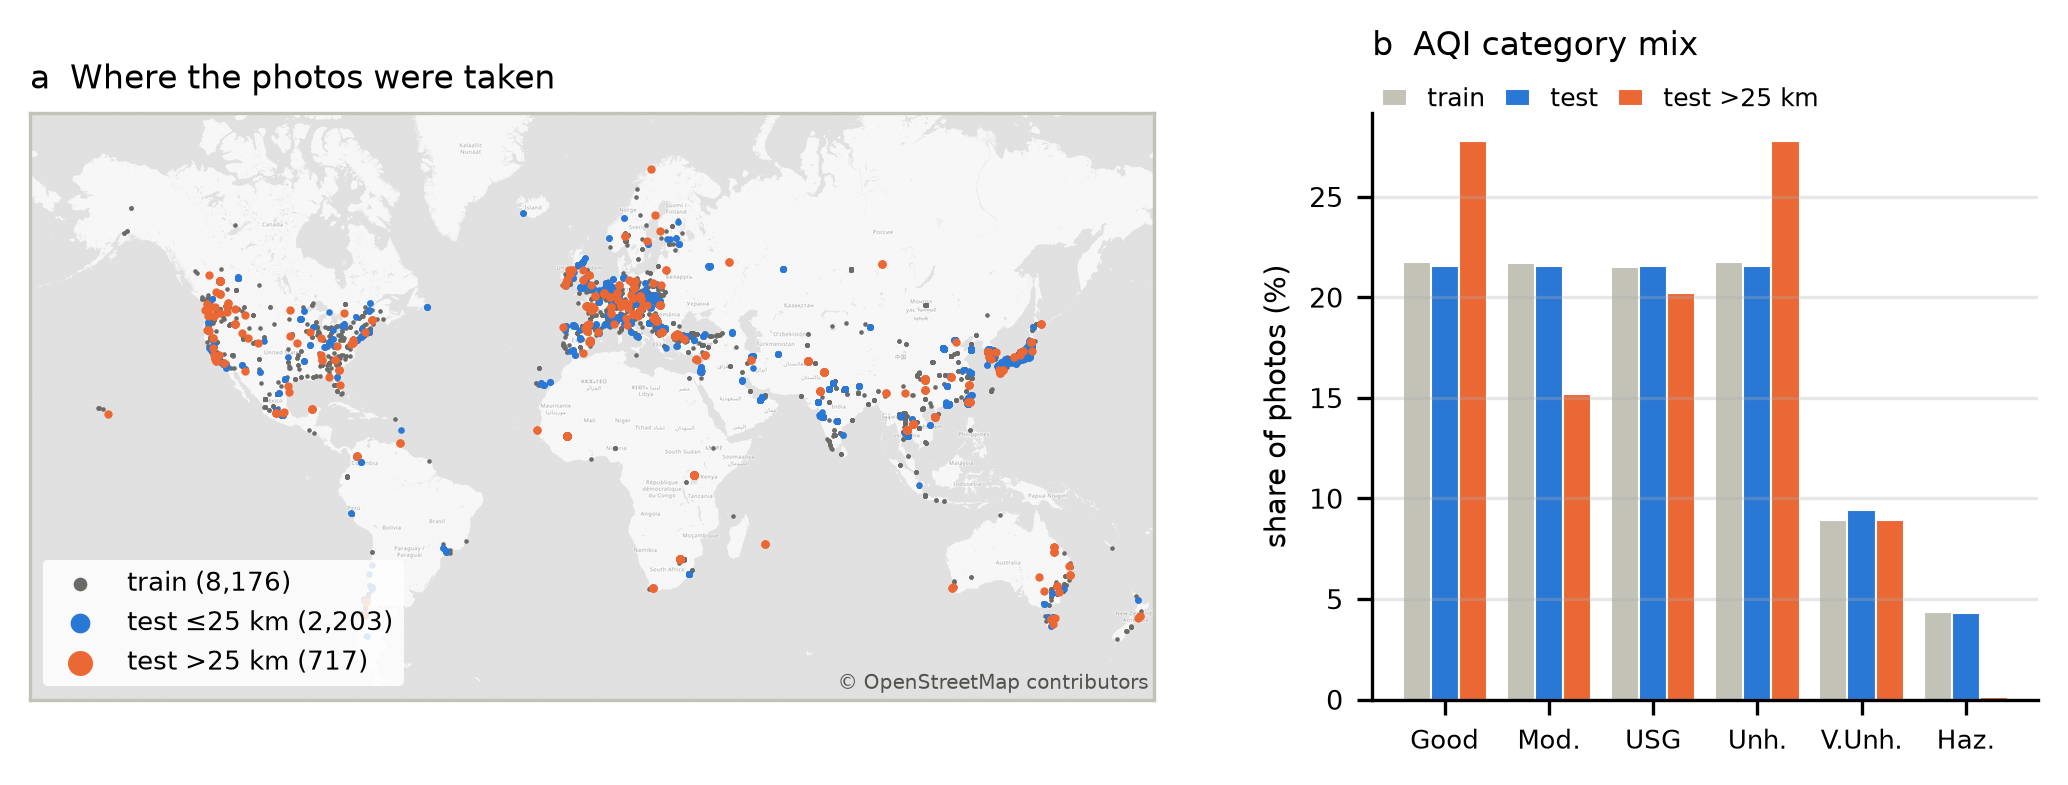
\includegraphics[width=\textwidth]{figures/final_dataset.png}
  \caption{(a) Locations of training photos (grey), test photos within 25~km of
  a training photo (blue) and the 717 unseen-region test photos (orange), on an
  OpenStreetMap basemap. (b) Share of each EPA category in each set.}
  \label{fig:dataset}
\end{figure*}

\subsection{Evaluation protocol}
Fixed cameras and dense city clusters make random splits misleading, so all
model selection used five-fold \texttt{StratifiedGroupKFold}, grouped either by
station or by spatial clusters of stations within 25~km (single-linkage on
Haversine distances), and stratified by AQI category. The number of training
epochs for each deep model was fixed from these cross-validation runs. Every
final model was then trained once on all 8,176 training images and its
\emph{last} epoch was evaluated exactly once on the test set. No test result was
used to choose anything.

We report two test sets: the full test set (2,920 photos, 729 stations) and
\texttt{test\_gt25km}, the 717 test photos (205 stations) that lie more than
25~km from every training photo. Three-quarters of the test photos lie within
25~km of a training photo, so the second set is the honest measure of
performance in a new region. Regression quality is measured by the mean
absolute error (MAE) in AQI points, root mean squared error, $R^2$ and Spearman
rank correlation; category quality by six-class accuracy, accuracy within one
category ($\pm$1 Acc), macro-F1, and the MAE on the two tail categories
(AQI$>$200). Because photos from one station are correlated, confidence
intervals come from a station-level cluster bootstrap: we resample stations with
replacement 1,000 times and recompute the MAE. Model comparisons use a
\emph{paired} station bootstrap of the MAE difference on identical resamples.

\subsection{Image processing: what the filters see}
Before training any network we asked which simple image operations respond to
pollution (notebook~2). Following Eq.~\eqref{eq:scatter} we computed six
per-pixel filter maps on each photo resized to 256$\times$192, with RGB values
$I^c\in[0,1]$:
\begin{align}
  \text{dark channel: } D(x) &= \min_{y\in\Omega_7(x)} \min_{c} I^c(y), \label{eq:dcp}\\
  \text{saturation: } S(x) &= \frac{\max_c I^c(x) - \min_c I^c(x)}{\max_c I^c(x) + \epsilon},\\
  \text{brightness: } V(x) &= \max_c I^c(x),\\
  \text{edges: } E(x) &= \sqrt{(G_x * Y)^2 + (G_y * Y)^2},\\
  \text{local contrast: } C(x) &= \operatorname{std}_{y\in\Omega_7(x)} Y(y),\\
  \text{blue ratio: } B(x) &= I^b(x) \,/\, \textstyle\sum_c I^c(x),
\end{align}
where $Y$ is the grey image, $G_x, G_y$ are Sobel kernels and $\Omega_7(x)$ is
a $7\times7$ window. Haze raises the dark channel and brightness and lowers
saturation, edges and local contrast. Because haze grows with distance, which
is largest near the horizon, we summarised every map over three horizontal
bands (top, middle, bottom) with the mean and the 10th and 90th percentiles,
giving 54 band features per photo. A second, physics-oriented set of 18
statistics (saturation, gradient and dark channel; mean and standard deviation
over the full image, top and bottom band) is computed in PyTorch by
\texttt{src/features/haze\_features.py}.

Fig.~\ref{fig:filters} shows why these filters are useful but not sufficient.
The top photo is grey and overcast and its haze maps look ``polluted'', yet the
AQI is 9; the bottom photo looks fairly clear and has an AQI of 302. On the
training set the single strongest feature, the 90th percentile of saturation in
the top band, has a Spearman correlation of only $-0.26$ with AQI. The
strongest signals come from the top band, which supports the distance argument
above (Fig.~\ref{fig:filtercorr}): saturation, edges, local contrast and the blue
ratio fall with AQI in the top band, the dark channel rises, and the bottom band,
dominated by nearby road, carries almost no signal. These findings shaped every
later model: the filters were built into
the first layer of our from-scratch CNNs, the 4-scalar physics prior was tested
inside PFRML, and we never apply brightness, contrast, saturation or hue
augmentation, because that would erase the signal.

\begin{figure*}[!t]
  \centering
  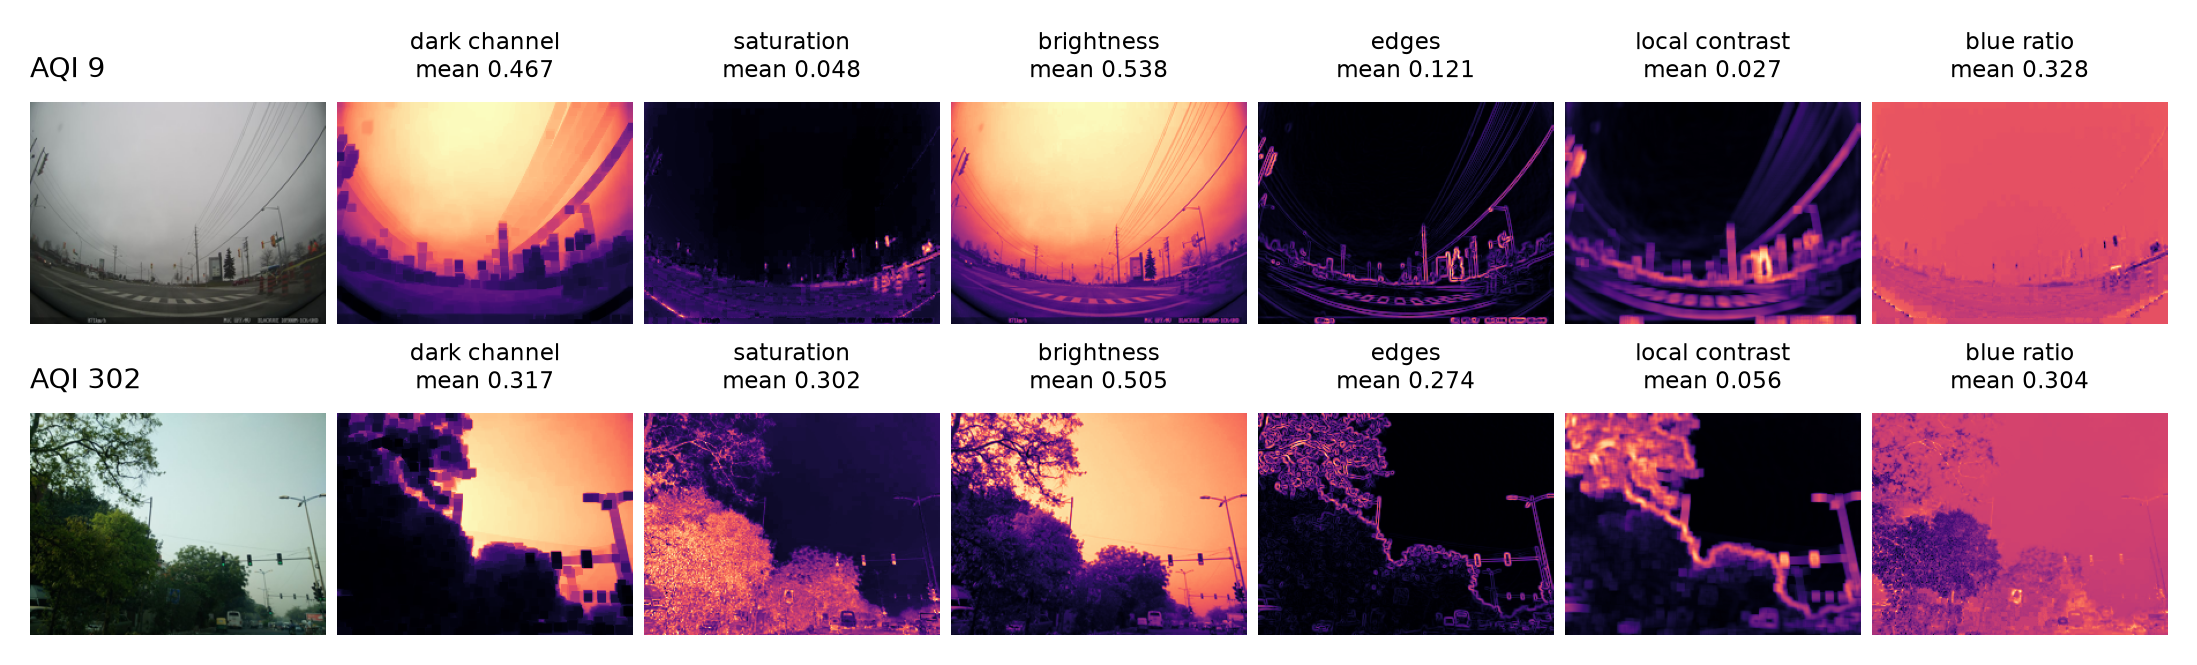
\includegraphics[width=\textwidth]{figures/final_haze_filters.png}
  \caption{The six haze filters on two training photos. Top: an overcast scene
  with AQI~9 looks hazy to every filter. Bottom: a scene with AQI~302 looks
  relatively clear. Grey sky is not the same as polluted air, which is why
  filters alone reach only $R^2=0.18$ (Table~\ref{tab:main}).}
  \label{fig:filters}
\end{figure*}

\begin{figure}[!t]
  \centering
  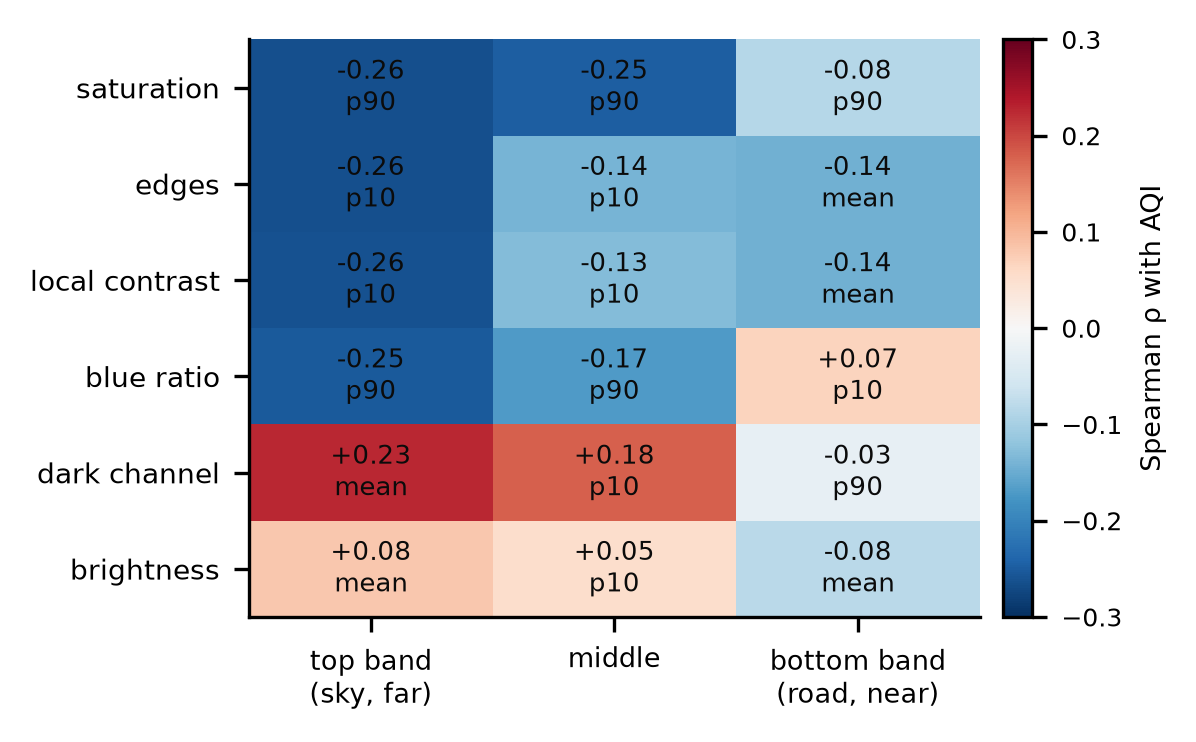
\includegraphics[width=\columnwidth]{figures/final_filter_corr.png}
  \caption{Strongest Spearman correlation with AQI for each filter and image
  band (training photos; the statistic that achieves it is printed below the
  value). Haze shows in the upper, distant part of the scene.}
  \label{fig:filtercorr}
\end{figure}

\subsection{Metadata encoding}
The only non-image inputs a phone can always provide are its position and the
date. We encode latitude $\varphi$, longitude $\lambda$ and month $m$ as
\begin{equation}
  z = \bigl[\cos\varphi\cos\lambda,\ \cos\varphi\sin\lambda,\ \sin\varphi,\
  \sin\tfrac{2\pi m}{12},\ \cos\tfrac{2\pi m}{12}\bigr],
  \label{eq:meta}
\end{equation}
a point on the unit sphere plus a cyclic month, so that neighbouring places and
December/January are close. We deliberately exclude concurrent sensor readings,
which a phone does not have and which let models skip the image
\cite{abdelsalamSkyFuseNetCrossAttentionSwin2026}.

% =====================================================================
\section{Models}\label{sec:models}
% =====================================================================

We trained nine models of increasing capacity, summarised in
Table~\ref{tab:main}. All deep models predict AQI$/100$ and use whole-image
resizing, so that both sky and ground stay in view, together with gentle
geometric augmentation (horizontal flip, $\pm5^\circ$ rotation, 2\% translation,
2\% scale for the 224-pixel models; flip and shifts of up to 8 pixels for the
small CNNs).

\subsection{Baselines}
\textbf{Median} predicts the training median (AQI~111) for every photo. It is
the floor any useful model must beat. \textbf{Ridge (18 haze stats)} and
\textbf{Ridge (54 band filters)} fit standardised linear regressions on the two
filter sets from Section~\ref{sec:data}, with the penalty chosen by internal
cross-validation for the first. \textbf{Metadata MLP} sees no pixels at all: a
5--64--32--1 network with ReLU on $z$ from Eq.~\eqref{eq:meta}, trained for 40
epochs with mean squared error. It measures how much of the task can be solved
by knowing \emph{where} and \emph{when} a photo was taken.

\subsection{From-scratch CNNs with built-in haze filters}
Notebook~3 builds two CNNs that receive the photo at 144$\times$192 pixels.
Their first layer is a fixed, differentiable \texttt{HazeFilters} module that
appends five filter maps (dark channel, saturation, brightness, Sobel edges,
local contrast) to the RGB channels, giving eight input channels.
\textbf{HazeCNN} (0.60\,M parameters) stacks four convolutional blocks with
batch normalisation and max-pooling, global average pooling and a small
head. \textbf{ResSE} (1.19\,M parameters) adds residual blocks and two
squeeze-and-excitation blocks, which learn one weight per channel so that
haze-related channels can be amplified. Both are trained with the L1 loss and
Adam, for 10 and 20 epochs respectively, with a cosine learning-rate decay.

\subsection{Pretrained MobileNetV3-Small}
\textbf{MobileNetV3-S} replaces the classifier of an ImageNet-pretrained
MobileNetV3-Small \cite{howard2019mobilenetv3} with a single regression output
(1.52\,M parameters). It is trained for 30 epochs with mean squared error,
AdamW (learning rate $10^{-3}$, weight decay $10^{-4}$), three warm-up epochs
and cosine decay, gradient clipping at 1.0 and batch size 32. This is the
simplest phone-ready image model and our main image-only reference.

\subsection{PFRML}
\textbf{PFRML full} follows the PFRML design
\cite{wangPrototypeFeatureRepresentationGuided2026} on the MobileNetV3-S spine.
Feature maps from four backbone stages are projected by $1\times1$
convolutions to $D{=}224$ channels, aligned to a $14\times14$ grid and summed
(the Dimension Consistency Module, DCM). A light two-layer, four-head
Transformer encodes the 196 tokens into an image embedding $\chi\in\mathbb{R}^{224}$.
Six class prototypes $p_k$ on the unit hypersphere, updated by an exponential
moving average, give class probabilities
$P(k\mid\chi) = \operatorname{softmax}_k\bigl(\cos(\chi,p_k)/\tau\bigr)$, and
the regression head receives $\chi$ together with the probability-weighted
prototype $\sum_k P(k\mid\chi)\,p_k$. The loss is
$\mathcal{L} = \mathcal{L}_{\mathrm{CE}}^{\epsilon} + \beta\,\mathcal{L}_{\mathrm{MSE}}$
with label smoothing $\epsilon{=}0.1$, $\beta{=}0.5$ and class weights
$w_k \propto N_k^{-0.5}$. The full variant also enables attention pooling over
the tokens and a sigmoid-gated physics prior built from four optical scalars
(luminance entropy, RMS contrast, dark-channel transmission $t$ and extinction
$-\ln t$). It is trained for 30 epochs.

\subsection{Fusion R1 (our deployed model)}
\textbf{Fusion R1} keeps the DCM and Transformer of PFRML but removes the
prototype branch, which our cross-validation showed hurt regression, and adds
the metadata branch (Fig.~\ref{fig:pipeline}A). With backbone $B$, neck $N$,
Transformer $T$ and metadata encoder $g$:
\begin{align}
  \chi &= T\bigl(N(B(x))\bigr) \in \mathbb{R}^{224}, \qquad m = g(z) \in \mathbb{R}^{32},\\
  \hat{y} &= 100\cdot h\bigl([\chi;\, m]\bigr),
\end{align}
where $h$ is a 256--256--1 MLP. An auxiliary head $h_{\mathrm{aux}}$ predicts
AQI from $\chi$ alone, with its gradient kept out of the metadata branch, so
that the image path must stay useful on its own:
\begin{equation}
  \mathcal{L} = \bigl\|h([\chi;m]) - \tfrac{y}{100}\bigr\|^2 + 0.5\,\bigl\|h_{\mathrm{aux}}(\chi) - \tfrac{y}{100}\bigr\|^2 .
\end{equation}
Fusion R1 has 2.02\,M parameters. It is trained with the same optimiser as
MobileNetV3-S for 7 epochs, a number fixed beforehand by a rule on the
spatial-cluster cross-validation curves. At test time we also evaluate it with
$m$ set to zero (\emph{metadata off}) to measure how much it depends on location,
and read out the auxiliary head, which is a free image-only prediction from the
same network. Fig.~\ref{fig:curves} shows the training curves of the five
neural models.

\begin{figure*}[!t]
  \centering
  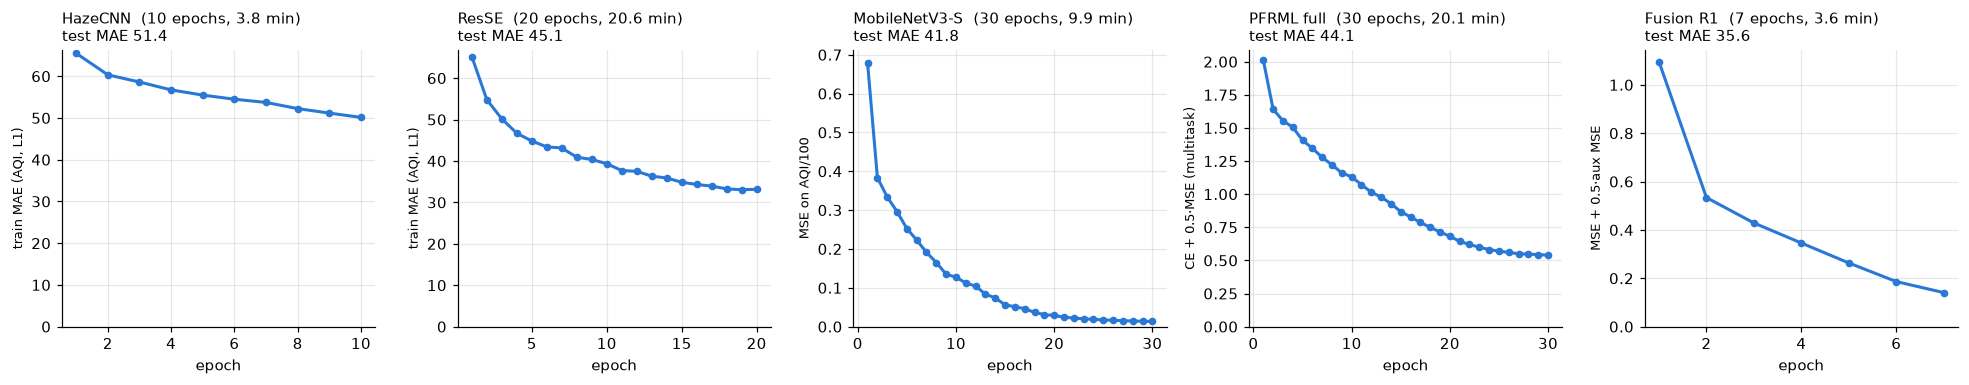
\includegraphics[width=\textwidth]{figures/final_nb4_training_curves.png}
  \caption{Training loss per epoch of the five neural models, each in its own
  loss units (no test data is used during training). MobileNetV3-S drives its
  training error far below its test error, a sign of overfitting that the fixed
  epoch budgets limit; HazeCNN is still improving after 10 epochs.}
  \label{fig:curves}
\end{figure*}

\begin{figure*}[!t]
  \centering
  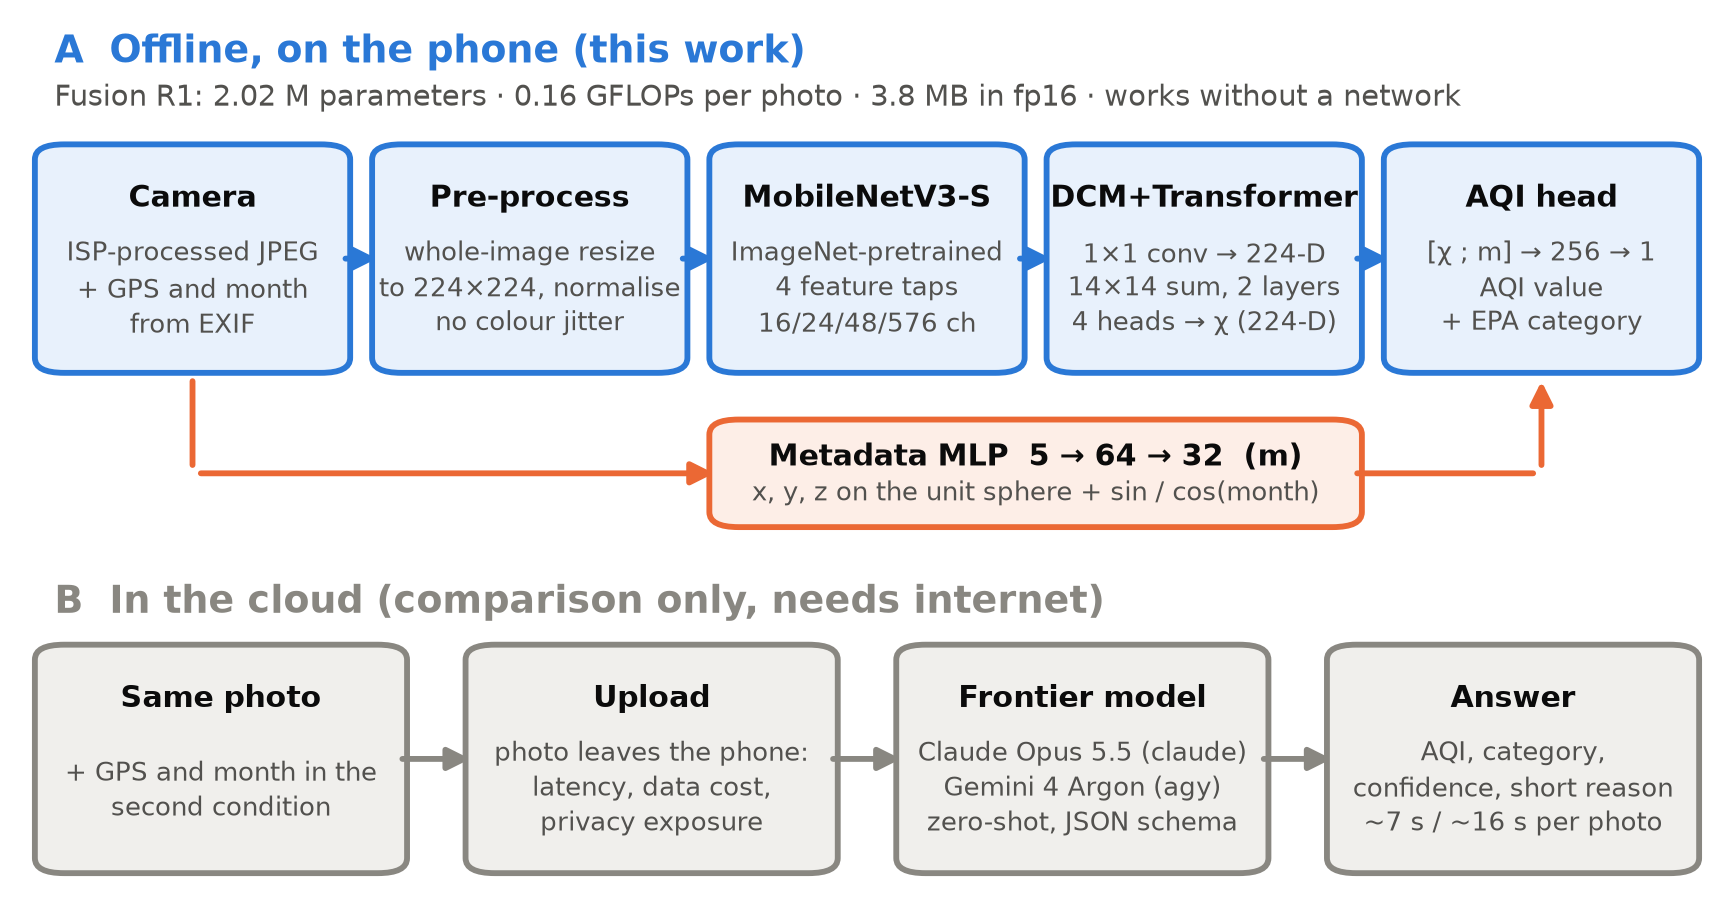
\includegraphics[width=0.92\textwidth]{figures/final_pipeline.png}
  \caption{(A) The offline pipeline: the photo and its GPS/month metadata are
  processed entirely on the phone by Fusion R1. (B) The cloud alternative we
  compare against: the same inputs are uploaded to a frontier model through its
  command-line agent.}
  \label{fig:pipeline}
\end{figure*}

% =====================================================================
\section{Frontier Models as Zero-Shot Estimators}\label{sec:frontier}
% =====================================================================

Because this work targets offline inference, frontier models cannot form part
of the proposed system: they are served from remote data centres, require
network connectivity, receive the user's image and location, and incur a
per-query cost. They nevertheless provide the natural reference point. If a
general-purpose model already estimates AQI accurately from a photograph, a
specialised offline model is justified only if it approaches that accuracy.

\subsection{Agents}
Two commercial multimodal models were evaluated as zero-shot AQI estimators.
Each was accessed through its vendor's command-line agent in non-interactive
(print) mode, authenticated with a standard user subscription rather than an
API key:
\begin{itemize}
  \item \textbf{Claude}: the Claude Code CLI (\texttt{claude -p}) with model
        \texttt{claude-opus-5-5} \cite{anthropic2026claude};
  \item \textbf{Gemini}: Google's Antigravity CLI (\texttt{agy -p}) with model
        \texttt{gemini-4-argon-medium} \cite{google2026gemini}.
\end{itemize}
For each query, the agent reads a single image file and returns a JSON object
validated against a fixed schema: an integer AQI in $[0,500]$, an EPA category,
a confidence in $[0,1]$ and a justification of at most 25 words. Notebook~5
(\texttt{5.frontier-and-mobile-deployment.ipynb}) issues the queries in
parallel via \texttt{subprocess}, retries failed calls and appends every raw
response to \texttt{results/frontier/predictions.jsonl}, which makes the
experiment resumable and fully auditable. Responses were collected on 21
November 2026 with Claude Code~2.1.330 at its default reasoning effort and
Antigravity~1.5.10; the identifier \texttt{gemini-4-argon-medium} selects
Gemini~4 Argon at the medium thinking level.

\subsection{Conditions and leakage control}
Each image is evaluated under two input conditions. In the \emph{photo only}
condition the prompt restricts the model to visible evidence (haze, contrast of
distant objects, sky colour), matching the information available to our
image-only models. In the \emph{photo + GPS + month} condition the prompt
additionally supplies the latitude and longitude (three decimals) and the month
of capture, and permits the use of prior knowledge about typical local air
quality; this corresponds exactly to the inputs of Fusion R1. The full prompts
are given in the Appendix.

Several controls prevent access to the ground truth. Each call executes in an
isolated directory that contains only the target image, renamed to its opaque
numeric identifier, so no metadata file is accessible. Claude is restricted to
the file-reading tool and therefore has no web access, and both agents are
instructed not to use any other tool or source. Only the month of capture is
disclosed, never the date, so the station reading for that day cannot be
retrieved. Session persistence is disabled, so no information carries over
between queries.

\subsection{Sample}
Given median response times of 6.7\,s (Claude) and 16.2\,s (Gemini) per query,
the evaluation uses a random sample of 200 test photos (seed 42) instead of the
full set of 2,920. All of our models are scored on the same 200 photos, so
every comparison is paired. The
sample comes from 150 stations and follows the test set: 49 Good, 57 Moderate,
43 USG, 29 Unhealthy, 19 Very Unhealthy and 3 Hazardous photos, 39 of them more
than 25~km from any training photo. All 800 queries (200 photos, two agents, two
conditions) returned a valid answer on the first attempt.

% =====================================================================
\section{Results}\label{sec:results}
% =====================================================================

All numbers in this section come from two notebooks:
\texttt{4.models-eval-and-result.ipynb} trains and scores every model under the
protocol of Section~\ref{sec:data}, and \texttt{5.frontier-and-mobile-deployment.ipynb}
runs the frontier agents and the footprint, distance and occlusion analyses on
notebook~4's saved models. Six of the models had been trained before with the same
recipes; our rerun reproduces five of them within 1~AQI point of their
recorded test MAE. The exception is the Metadata MLP, discussed below (the
metadata-off ablation of Fusion R1 also moved, by 3.0).

\begin{table*}[!t]
  \centering
  \caption{All models on the full test set (2,920 photos, 729 stations) and on
  the unseen-region subset (717 photos $>$25~km from any training photo),
  sorted by test MAE. Brackets: 95\% station-bootstrap CI. Tail MAE: photos with
  AQI$>$200. Lower MAE and higher $R^2$/accuracy are better.}
  \label{tab:main}
  \setlength{\tabcolsep}{4pt}
  \begin{tabular}{llrcccccccc}
    \toprule
    & & & \multicolumn{6}{c}{Full test set} & \multicolumn{2}{c}{Unseen regions ($>$25~km)} \\
    \cmidrule(lr){4-9}\cmidrule(lr){10-11}
    Model & Input & Params & MAE [95\% CI] & $R^2$ & Acc & $\pm$1 Acc & Tail MAE & & MAE [95\% CI] & $R^2$ \\
    \midrule
    \textbf{Fusion R1} & photo, GPS, month & 2.02\,M & \textbf{35.6} [30.2, 43.4] & \textbf{0.60} & \textbf{0.46} & \textbf{0.90} & 76 & & 39.3 [31.4, 46.7] & \textbf{0.38} \\
    Metadata MLP & GPS, month & 2,497 & 36.8 [31.5, 43.4] & 0.59 & 0.40 & 0.90 & \textbf{70} & & 48.6 [39.2, 57.2] & $-0.05$ \\
    MobileNetV3-S & photo & 1.52\,M & 41.8 [35.1, 50.6] & 0.44 & 0.41 & 0.85 & 95 & & \textbf{39.2} [28.2, 52.5] & 0.29 \\
    PFRML full & photo & 2.11\,M & 44.1 [36.9, 53.4] & 0.32 & 0.42 & 0.83 & 97 & & 46.5 [35.5, 57.0] & $-0.02$ \\
    Fusion R1, metadata off & photo & 2.02\,M & 44.6 [37.5, 54.5] & 0.42 & 0.36 & 0.82 & 106 & & 43.8 [32.6, 55.7] & 0.20 \\
    ResSE & photo & 1.19\,M & 45.1 [37.0, 56.3] & 0.36 & 0.38 & 0.82 & 111 & & 43.5 [30.4, 59.8] & 0.08 \\
    HazeCNN & photo & 0.60\,M & 51.4 [43.4, 63.0] & 0.26 & 0.31 & 0.77 & 128 & & 45.7 [34.6, 60.5] & 0.10 \\
    Ridge (54 band filters) & filters & 55 & 54.8 [46.7, 67.0] & 0.18 & 0.27 & 0.76 & 121 & & 50.0 [41.8, 60.8] & 0.07 \\
    Ridge (18 haze stats) & filters & 19 & 60.8 [52.0, 73.9] & 0.04 & 0.23 & 0.68 & 141 & & 53.8 [44.9, 66.5] & $-0.04$ \\
    Median & -- & -- & 63.6 [54.2, 77.0] & $-0.01$ & 0.22 & 0.65 & 156 & & 56.6 [48.7, 66.9] & $0.00$ \\
    \bottomrule
  \end{tabular}
\end{table*}

\subsection{Overall accuracy (RQ1)}
Table~\ref{tab:main} and Fig.~\ref{fig:mae} give the full picture. Fusion R1 is
the most accurate model on the full test set, with an MAE of 35.6 and
$R^2=0.60$, against 63.6 for the constant median. It places 46\% of photos in
the exact EPA category and 90\% within one category.

The ranking also shows what each ingredient adds. Handcrafted haze filters on
their own explain little ($R^2$ 0.04--0.18), which confirms the ambiguity of
Fig.~\ref{fig:filters}. Learning convolutional features on top of the same
filters helps: HazeCNN reaches 51.4 and the deeper ResSE 45.1. ImageNet
pretraining helps more. MobileNetV3-S reaches 41.8 while needing 17--54 times
less compute than the two from-scratch CNNs (Table~\ref{tab:footprint}). The
PFRML prototype branch does \emph{not} help: PFRML full (44.1) is worse than
the plain MobileNetV3-S it is built on, and its predictions snap to a few
prototype levels, visible as horizontal bands in a predicted-versus-true plot.
Adding location and month to the image path is the largest single gain: Fusion
R1 is 6.1 points better than MobileNetV3-S.

Fig.~\ref{fig:scorecard} ranks every model on every metric at once, including
its cost per photo, and Fig.~\ref{fig:predtrue} shows the predictions
themselves. The two Ridge models and the median produce a flat cloud around the
mean, the from-scratch CNNs begin to follow the diagonal, and the pretrained
models follow it until about AQI~200, beyond which every model flattens out.

\begin{figure*}[!t]
  \centering
  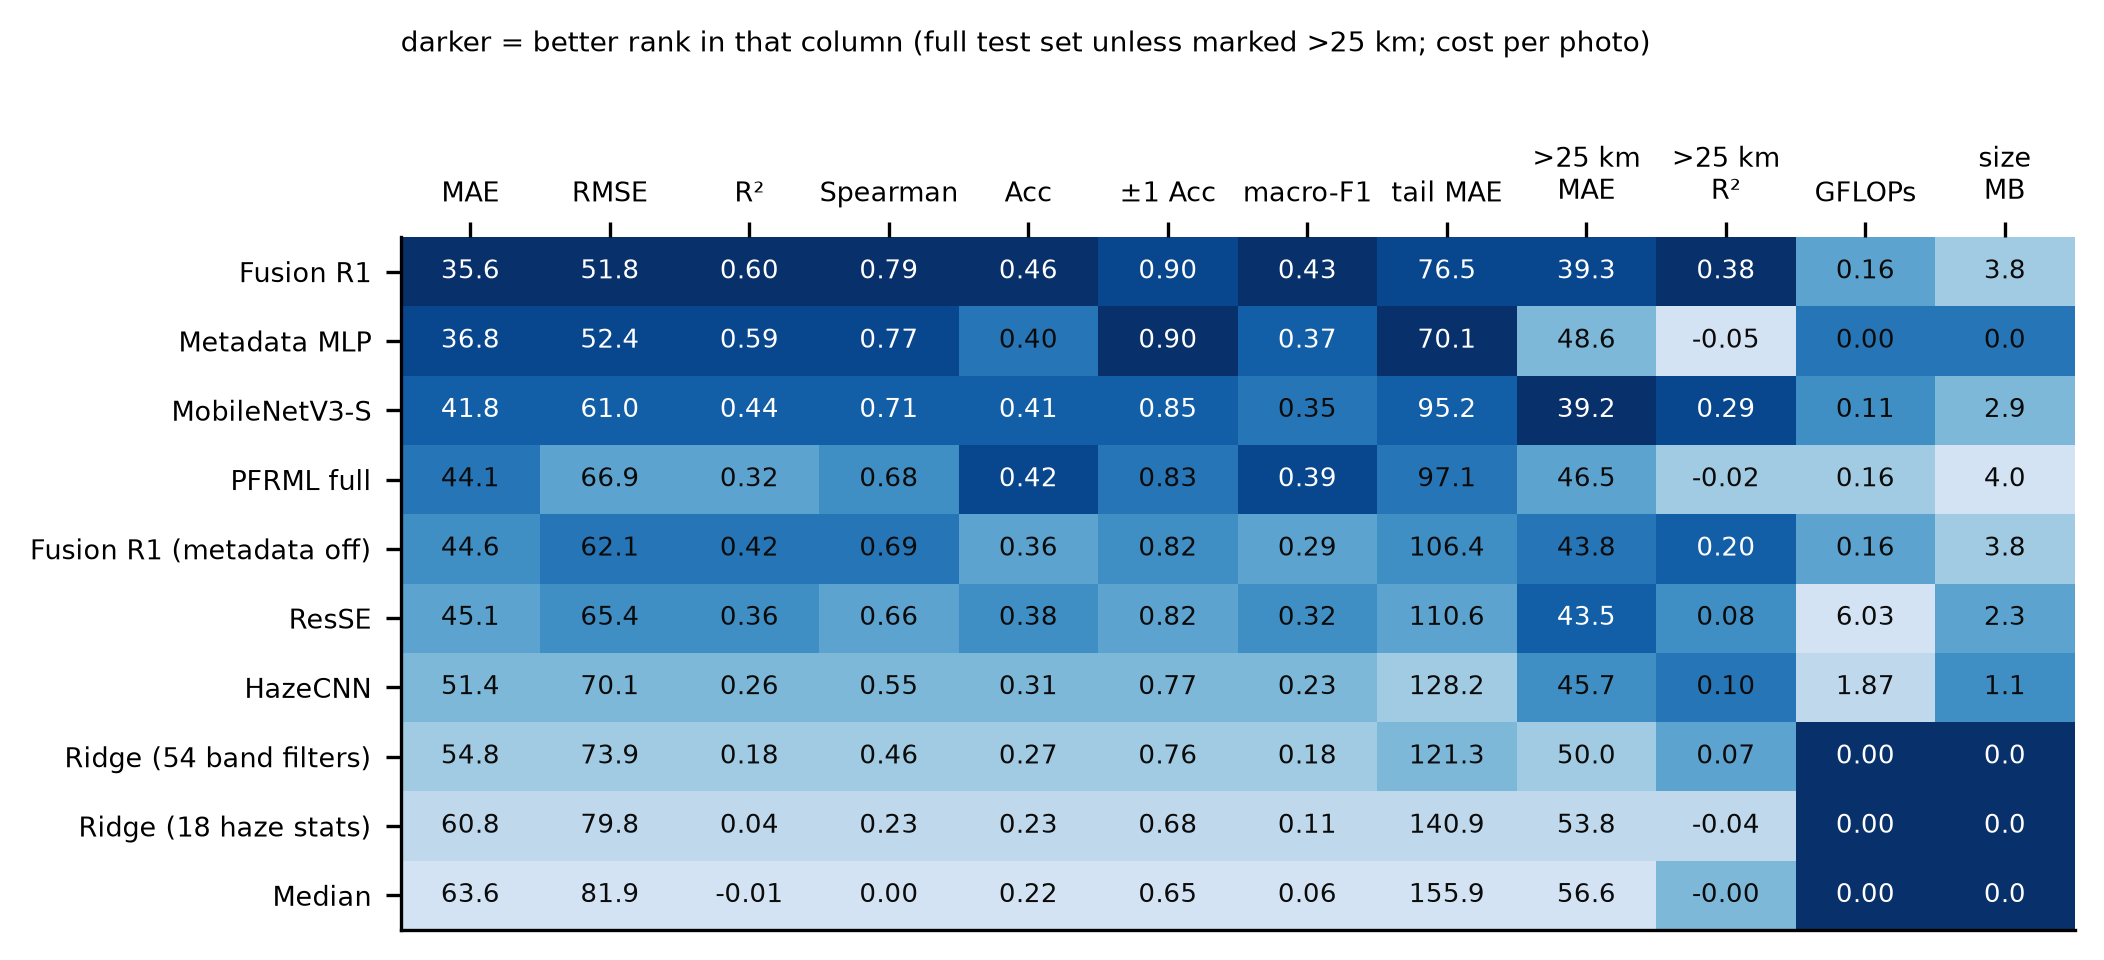
\includegraphics[width=\textwidth]{figures/final_scorecard.png}
  \caption{Scorecard of all models: every column is a metric (accuracy on the
  full test set unless marked $>$25~km; compute and fp16 weight size per photo),
  shaded by rank within the column. Fusion R1 ranks first or second on all ten
  accuracy metrics.}
  \label{fig:scorecard}
\end{figure*}

\begin{figure*}[!t]
  \centering
  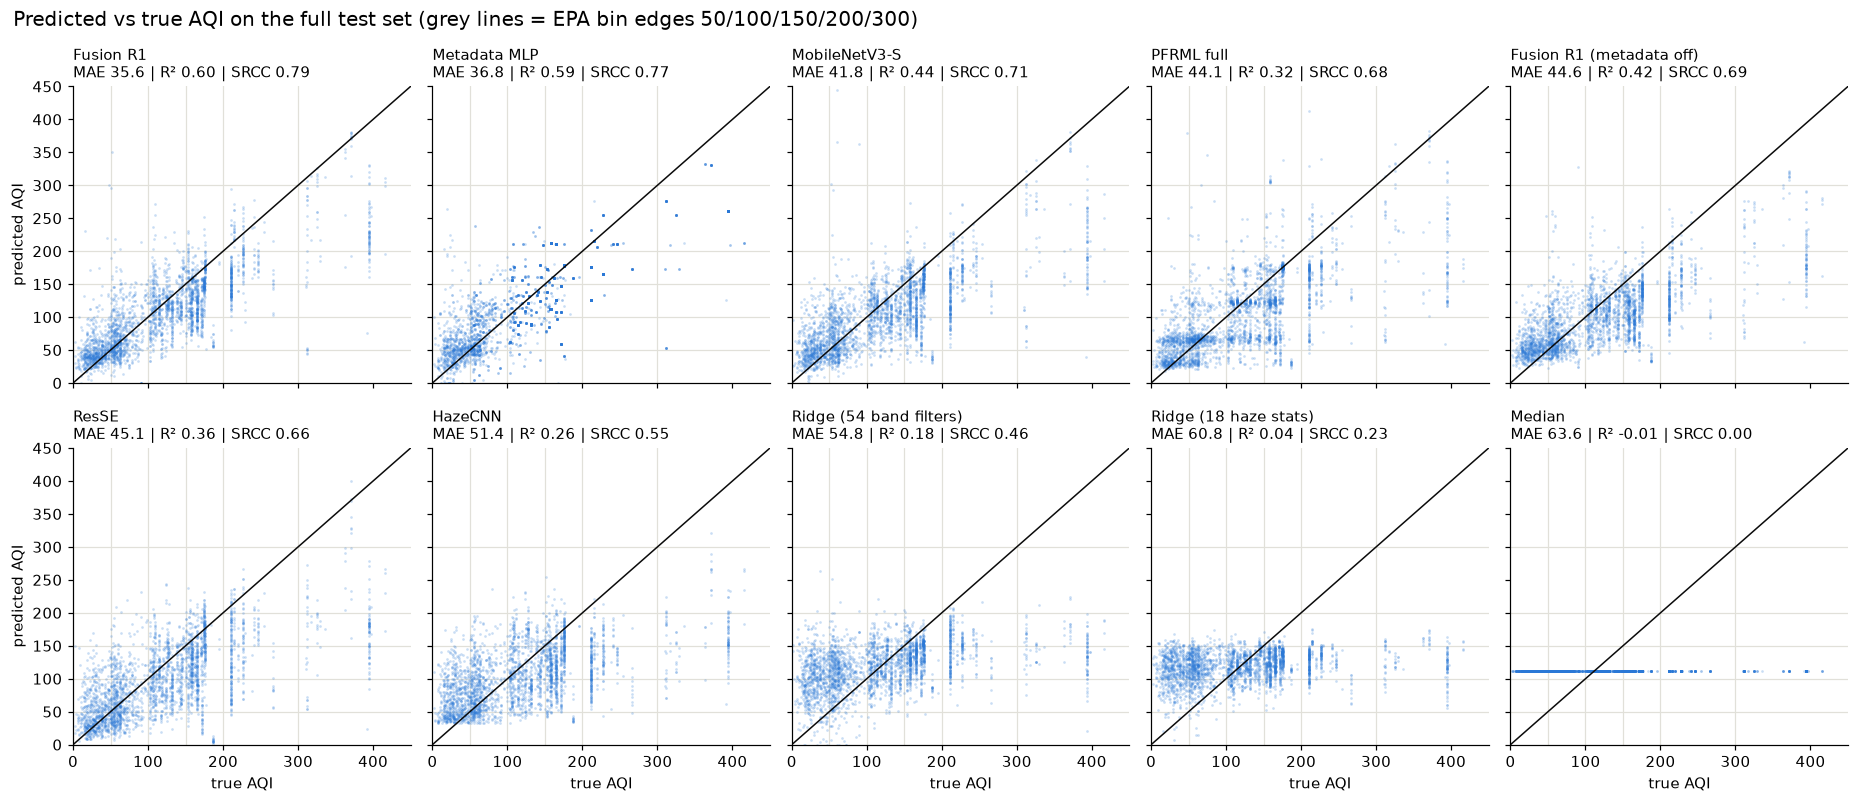
\includegraphics[width=\textwidth]{figures/final_nb4_pred_vs_true.png}
  \caption{Predicted versus true AQI for every model on the full test set.
  Grey lines mark the EPA category edges; a perfect model lies on the diagonal.
  PFRML's predictions snap to a few horizontal bands (prototype levels), and the
  Metadata MLP predicts nearly the same value for every photo of a station.}
  \label{fig:predtrue}
\end{figure*}

\begin{figure*}[!t]
  \centering
  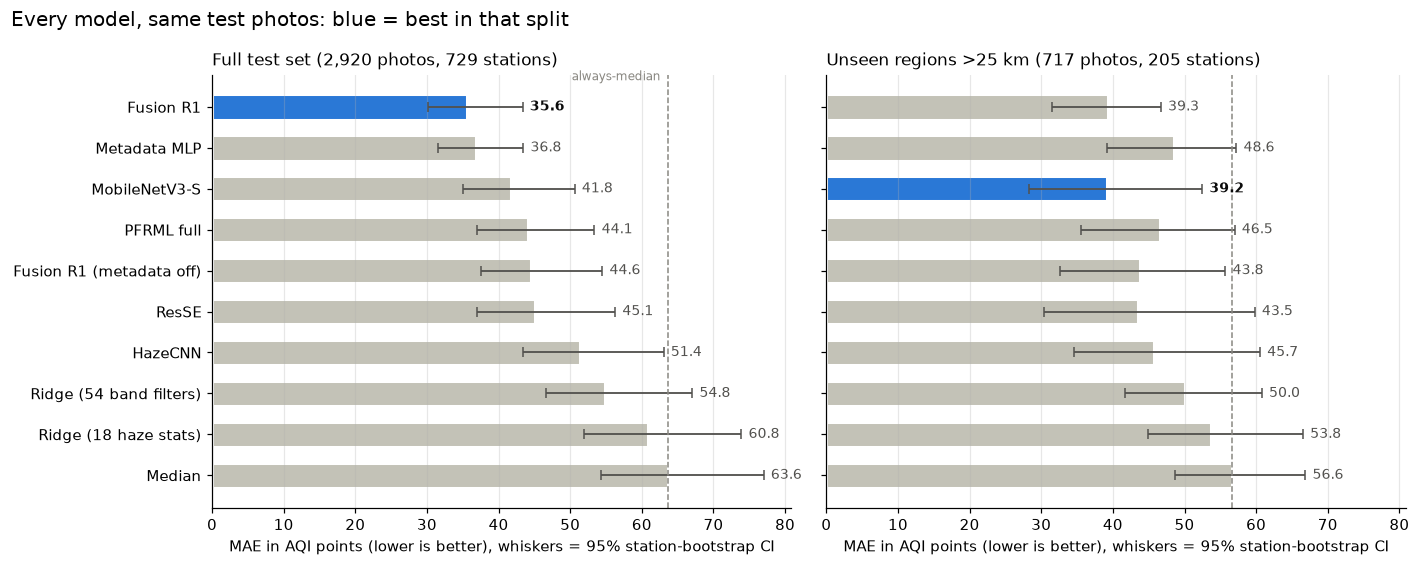
\includegraphics[width=0.95\textwidth]{figures/final_nb4_mae_comparison.png}
  \caption{Test MAE with 95\% station-bootstrap CIs for every model. Left: full
  test set. Right: photos more than 25~km from any training photo. Blue marks
  the best model in each panel; the dashed line is the constant-median baseline.}
  \label{fig:mae}
\end{figure*}

\subsection{Unseen regions and the metadata shortcut (RQ2)}
The Metadata MLP sees no pixels, yet on the full test set it comes within 1.2
points of Fusion R1 (36.8). Pollution is strongly regional and seasonal, and
three-quarters of the test photos were taken within 25~km of a training photo,
so ``the usual AQI here in this month'' is already a good answer. That answer
fails in a new region. Beyond 25~km the Metadata MLP falls to 48.6 with
$R^2=-0.05$, worse than predicting a constant, while Fusion R1 holds 39.3
($R^2=0.38$) and the image-only MobileNetV3-S holds 39.2. The ablation tells the
same story from inside one network: zeroing the metadata of the trained Fusion
R1 costs 8.9 MAE on the full test set but only 4.5 beyond 25~km.

Fig.~\ref{fig:distance} looks at distance in finer steps. Within 25~km of
training data the Metadata MLP is as good as Fusion R1. Beyond 100~km it falls
apart (60.7 between 100 and 500~km), while the image-only MobileNetV3-S becomes
the \emph{best} model (30.4 at 100--500~km, 27.3 beyond 500~km, against 37.8 and
44.2 for Fusion R1). The far bins are small (166 and 53 photos), but the
direction is clear: far from any training station the location prior misleads
the fusion model, and the photo alone is more reliable. The same pattern appears
by region (Fig.~\ref{fig:distance}b): the image-only model is strongest in Africa
and North America, where training stations are sparse, while location helps in
densely sampled Europe and Asia.

\begin{figure*}[!t]
  \centering
  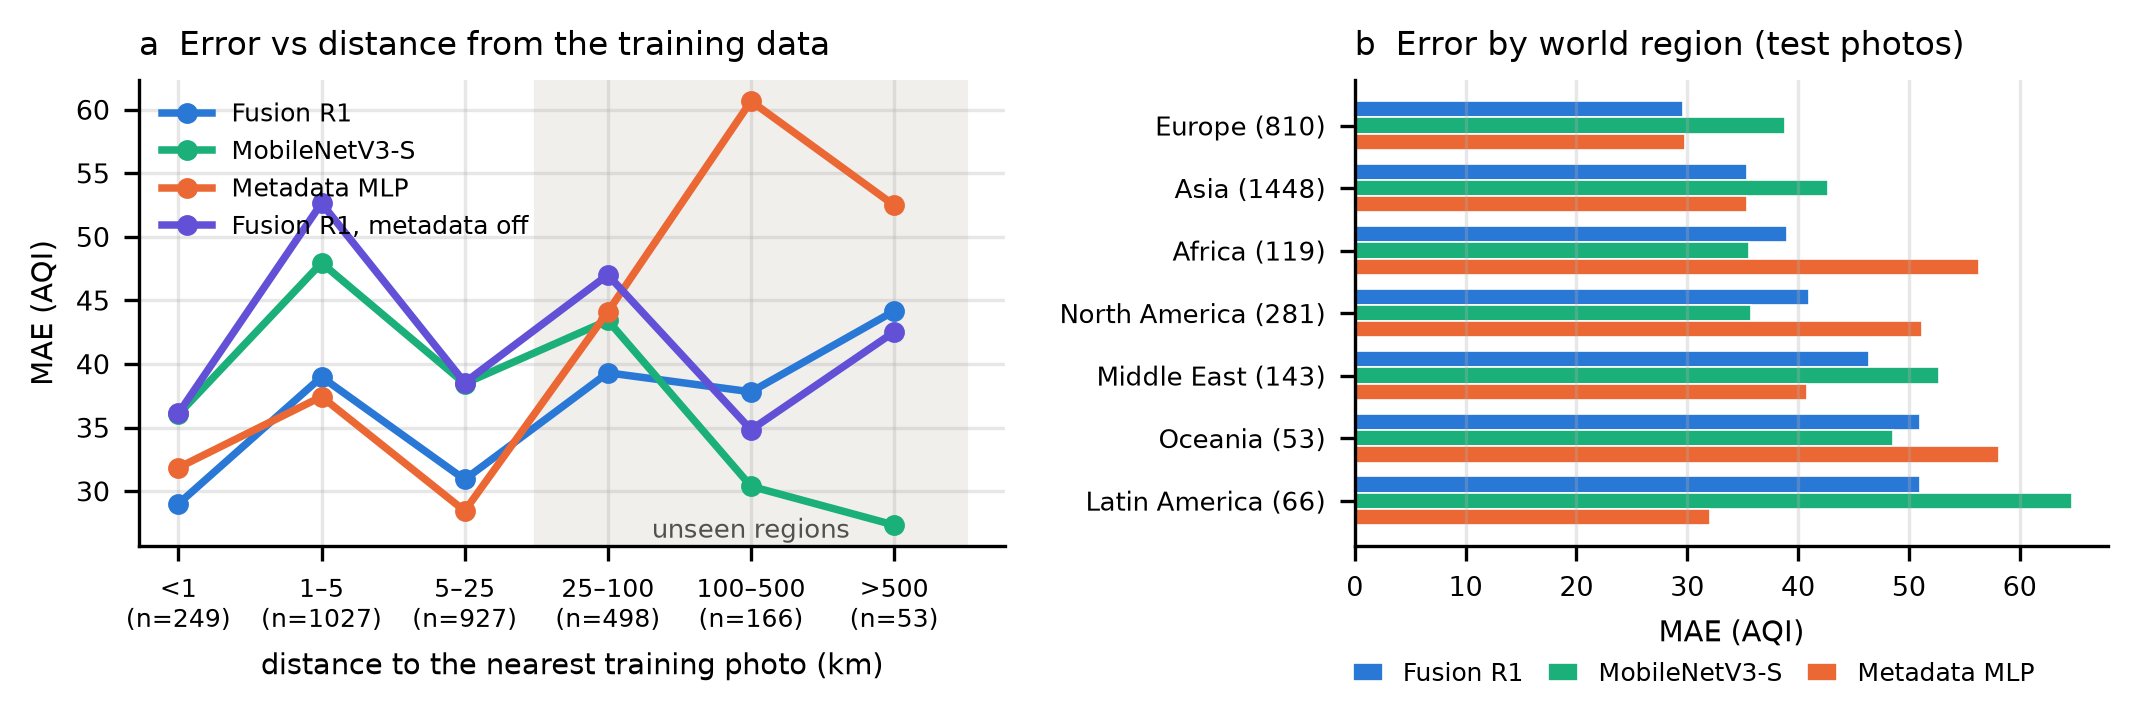
\includegraphics[width=\textwidth]{figures/final_distance_region.png}
  \caption{(a) Test MAE as a function of distance to the nearest training photo
  (the shaded part is the unseen-region subset). (b) Test MAE by world region
  (regions with at least 40 test photos; photo counts in brackets).}
  \label{fig:distance}
\end{figure*}

Fusion R1 can exploit this without a second model, because its auxiliary head
already predicts AQI from the image embedding alone. Over three seeds the
auxiliary head scores 42.2 on the full test set, the same as a separately
trained MobileNetV3-S, and 32.4 beyond 100~km, where the main head scores 40.0
(Fig.~\ref{fig:heads}). Simply zeroing the metadata of the main head is not a
substitute: it gives 44.6 to 55.0 depending on the seed, because the main head
never saw a zero embedding during training. A distance-aware switch, which uses
the main head near known stations and the image-only head beyond about 100~km,
is therefore a free improvement for a deployed app. We found the 100~km boundary
by looking at the test set, so it must be confirmed on held-out data before it
is used.

\begin{figure*}[!t]
  \centering
  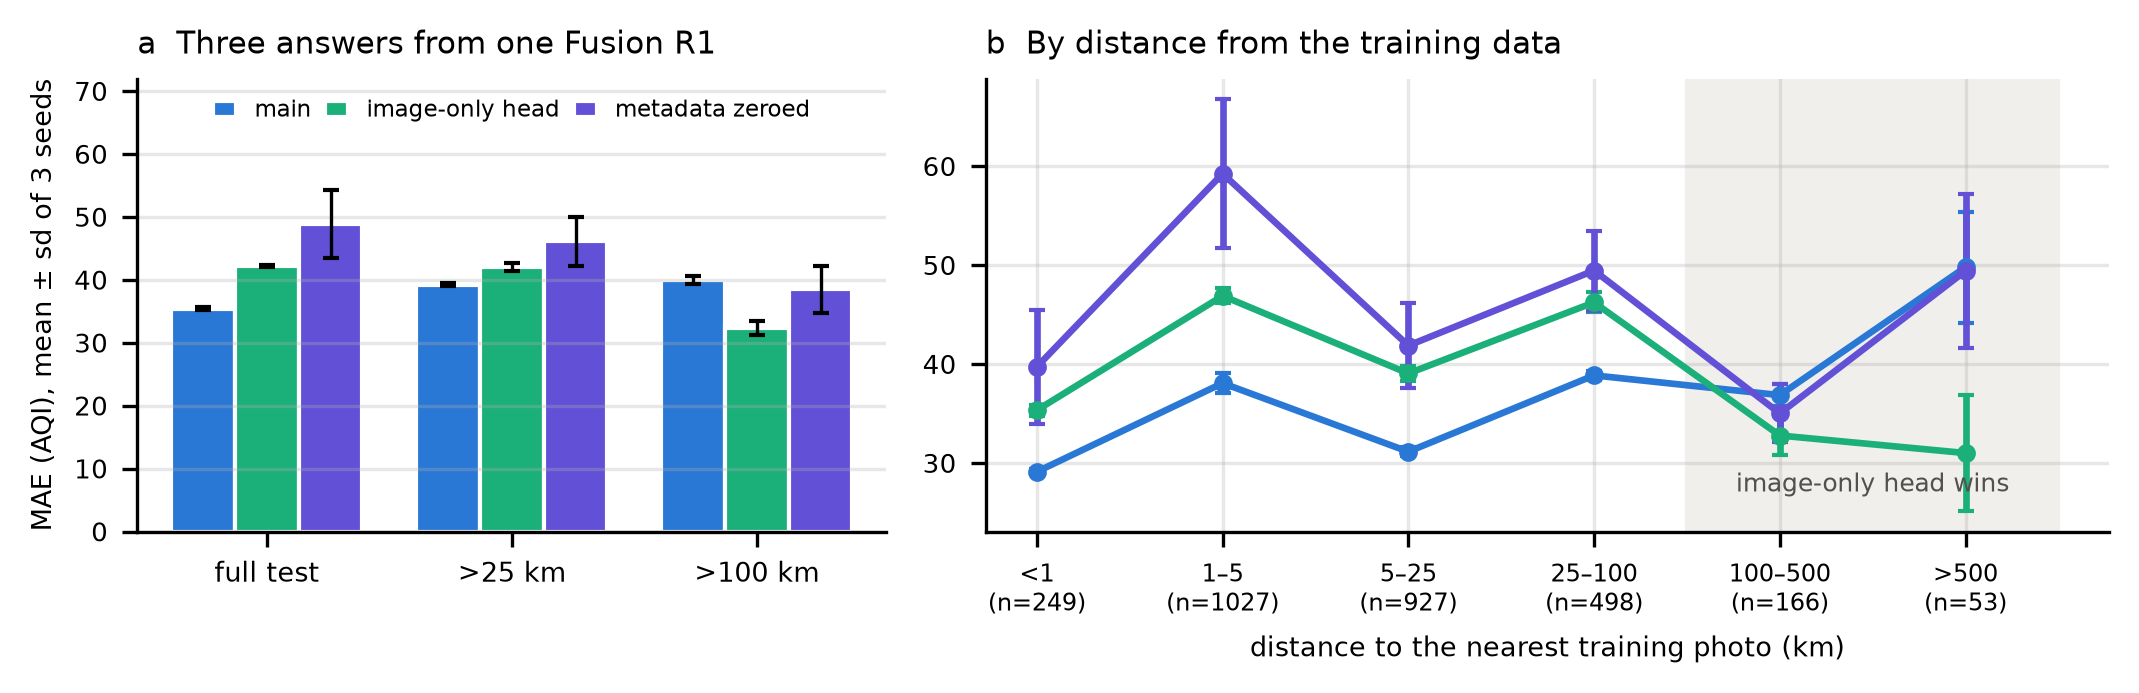
\includegraphics[width=\textwidth]{figures/final_fusion_heads.png}
  \caption{Three answers from one trained Fusion R1: the main head (photo, GPS
  and month), its built-in image-only auxiliary head, and the main head with the
  metadata zeroed. Bars and error bars: mean and standard deviation over three
  training seeds. Beyond 100~km the image-only head is the most accurate.}
  \label{fig:heads}
\end{figure*}

\begin{table}[!t]
  \centering
  \caption{Paired station bootstrap of MAE(other)$-$MAE(Fusion R1). Positive
  means Fusion R1 is more accurate; * the 95\% CI excludes zero. Seed-averaged
  rows average the predictions of 3 (Fusion R1, MobileNetV3-S) or 5 (Metadata
  MLP) training seeds.}
  \label{tab:paired}
  \setlength{\tabcolsep}{3pt}
  \begin{tabular}{lcc}
    \toprule
    Comparison & Full test & $>$25~km \\
    \midrule
    Metadata MLP, single run & $+1.2$ [$-2.3$, 4.5] & $+9.2$ [2.1, 16.3]* \\
    Metadata MLP, seed-averaged & $+1.6$ [$-1.6$, 4.7] & $+7.9$ [1.8, 13.8]* \\
    MobileNetV3-S, single run & $+6.1$ [3.5, 8.5]* & $-0.1$ [$-5.9$, 7.4] \\
    MobileNetV3-S, seed-averaged & $+6.4$ [3.5, 9.3]* & $+0.9$ [$-6.3$, 9.6] \\
    PFRML full, single run & $+8.5$ [5.5, 11.5]* & $+7.2$ [2.5, 11.3]* \\
    \bottomrule
  \end{tabular}
\end{table}

Table~\ref{tab:paired} tests these differences properly. No model is
significantly more accurate than Fusion R1 on either test set. Fusion R1 is
significantly better than the Metadata MLP in unseen regions and significantly
better than MobileNetV3-S on the full test set; in each of the other two cells
the difference is not significant. It is the only model that is at or near the
top on both test sets. Fig.~\ref{fig:paired} shows the same test for every model.

\begin{figure*}[!t]
  \centering
  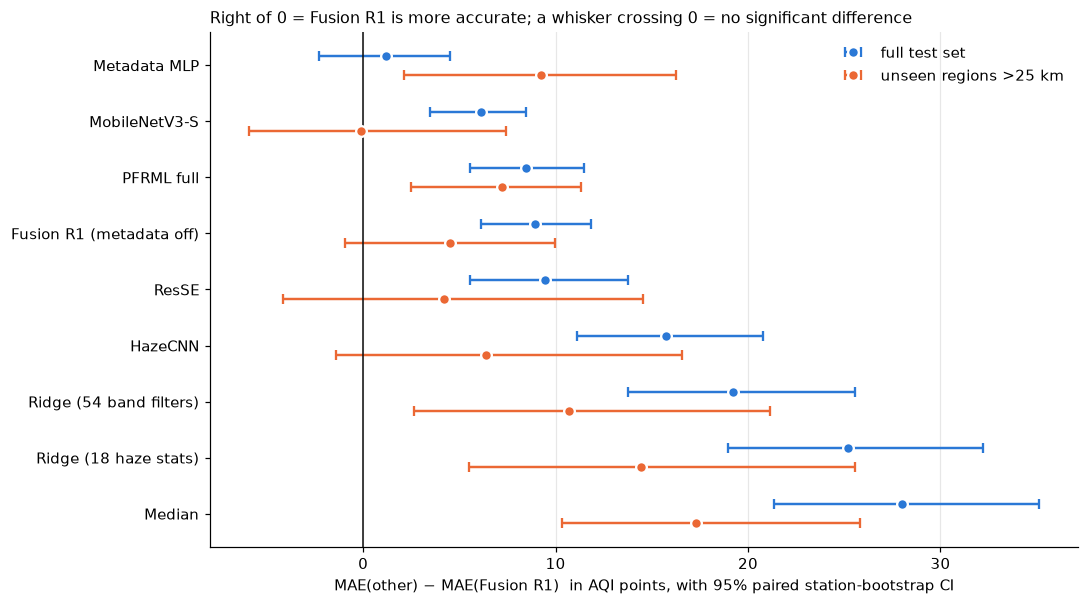
\includegraphics[width=0.72\textwidth]{figures/final_nb4_paired_bootstrap.png}
  \caption{Paired station bootstrap of MAE(other)$-$MAE(Fusion R1) on the full
  test set (blue) and beyond 25~km (orange). Right of zero means Fusion R1 is
  more accurate; a whisker crossing zero means no significant difference.}
  \label{fig:paired}
\end{figure*}

\subsection{Run-to-run variation}
A single training run is one random draw. The same Metadata MLP recipe scored
40.3 in an earlier recorded run and between 35.8 and 37.4 in five runs here, so
we retrained the three leading models with extra seeds (Fig.~\ref{fig:seeds}).
Fusion R1 is remarkably stable: $35.4\pm0.3$ on the full test set and
$39.2\pm0.2$ beyond 25~km over three seeds. MobileNetV3-S gives
$42.3\pm0.5$ and $41.4\pm2.0$, so its tie with Fusion R1 in unseen regions in
Table~\ref{tab:main} came from a favourable seed. The Metadata MLP gives
$36.6\pm0.6$ and $47.2\pm1.0$ over five seeds. Seed-averaged predictions lead to
the same conclusions as single runs (Table~\ref{tab:paired}). A practical lesson
is that single-run gaps below about 2 MAE should not be trusted on this dataset.

\begin{figure*}[!t]
  \centering
  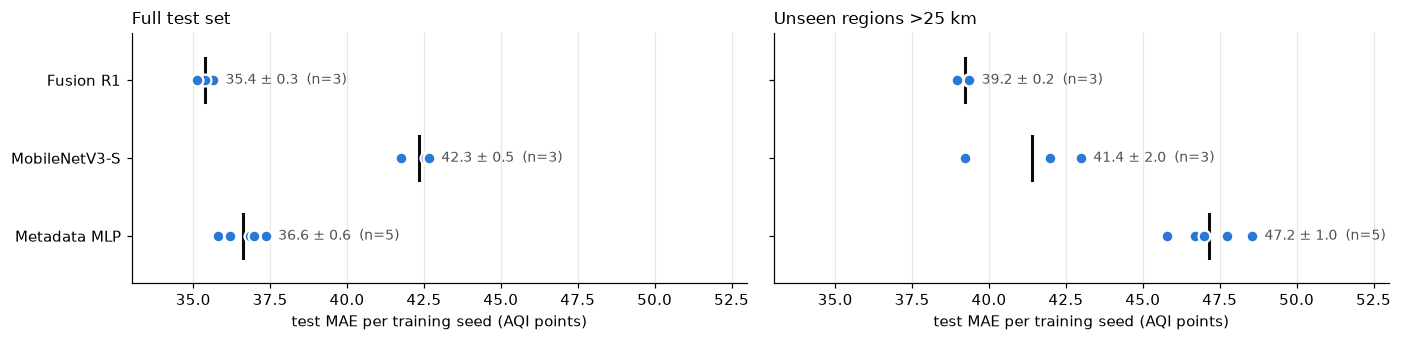
\includegraphics[width=0.85\textwidth]{figures/final_nb4_seed_robustness.png}
  \caption{Test MAE of every training seed (dots) and their mean (bar) for the
  three leading models. Fusion R1 varies by less than half an AQI point.}
  \label{fig:seeds}
\end{figure*}

\subsection{Where every model fails}
Fig.~\ref{fig:perbin} breaks the error down by true category. All models
over-predict clean air and under-predict polluted air; they regress towards the
middle of the scale. The effect is worst in the Hazardous category, where the
mean bias ranges from $-114$ (Metadata MLP) and $-126$ (Fusion R1) to $-241$
(Ridge on haze statistics). Only 355 training photos are that polluted,
and very high AQI often coincides with smoke or dust episodes whose look varies
widely. For a user this means the offline model is reliable as a coarse
indicator (clean, moderate, unhealthy), and that it will understate extreme
episodes. The six-class confusion matrices (Fig.~\ref{fig:confusion}) confirm
this: errors fall mostly in neighbouring categories, which is why $\pm$1 accuracy (90\%) is much higher than
exact accuracy (46\%).

\begin{figure*}[!t]
  \centering
  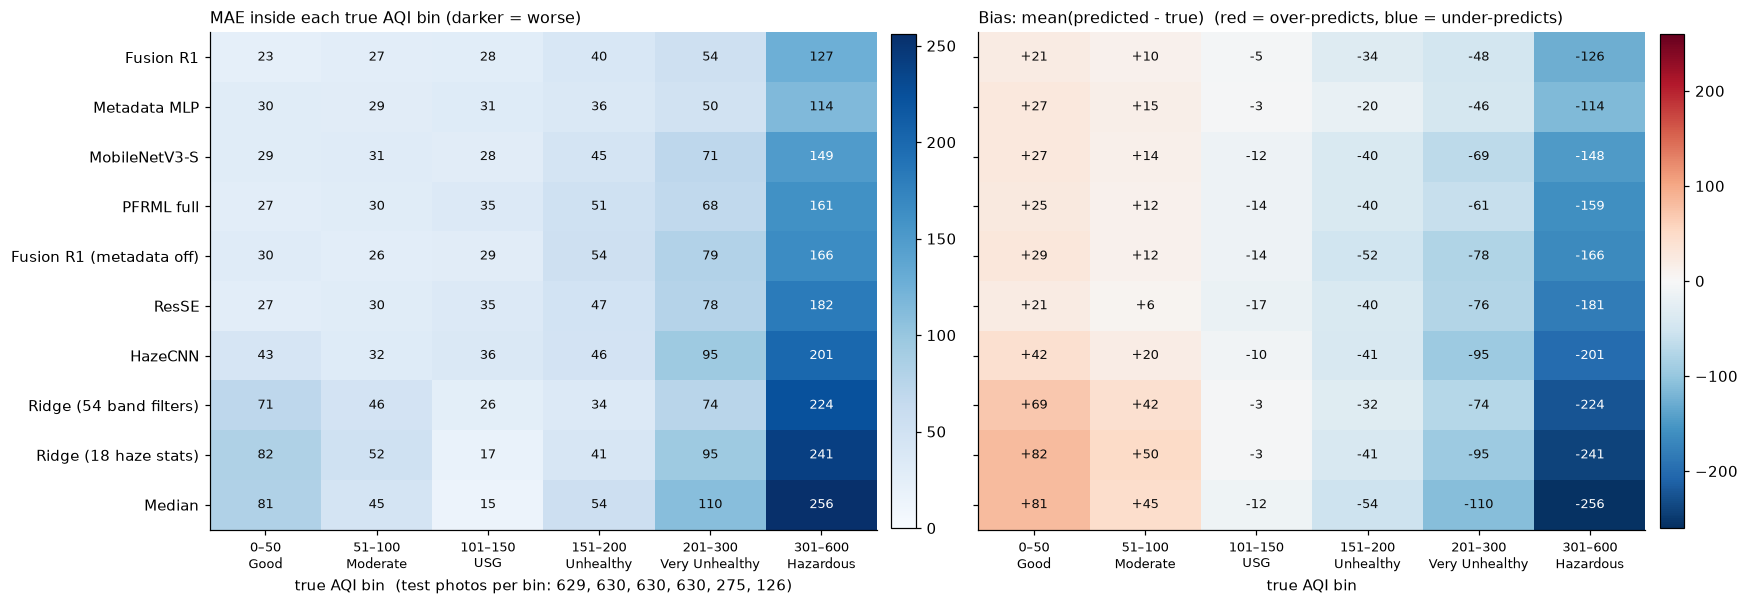
\includegraphics[width=\textwidth]{figures/final_nb4_per_bin_error.png}
  \caption{Left: MAE inside each true EPA category. Right: mean signed error
  (prediction $-$ truth). Every model over-predicts clean air (red) and
  under-predicts hazardous air (blue).}
  \label{fig:perbin}
\end{figure*}

\begin{figure*}[!t]
  \centering
  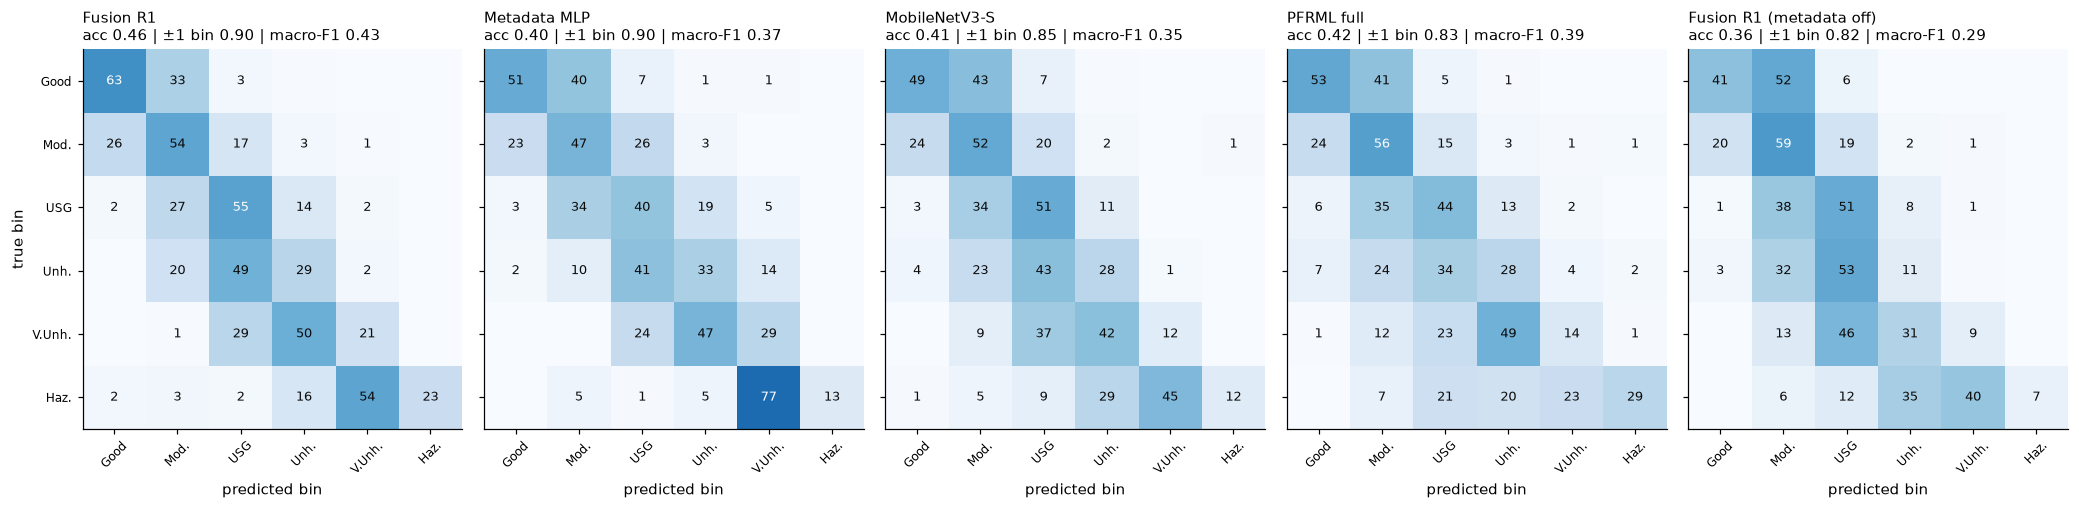
\includegraphics[width=\textwidth]{figures/final_nb4_confusion_top5.png}
  \caption{Six-class confusion matrices of the five best models (rows: true
  category, values: percent of the row). Most errors fall one category away
  from the truth; Hazardous photos are mostly called Very Unhealthy.}
  \label{fig:confusion}
\end{figure*}

\subsection{Frontier models versus our offline models (RQ3)}
Table~\ref{tab:frontier} and Fig.~\ref{fig:frontiermae} compare the four
frontier configurations with all our models on the same 200 test photos. Three
findings emerge.

\begin{table*}[!t]
  \centering
  \caption{Frontier agents and our offline models on the same 200 test photos
  (150 stations). Brackets: 95\% station-bootstrap CI. $\Delta$: paired
  station-bootstrap MAE difference to Fusion R1 (negative = better than Fusion
  R1); * CI excludes zero. Bias: mean(predicted$-$true). The last column covers
  only the 39 photos more than 25~km from training data.}
  \label{tab:frontier}
  \setlength{\tabcolsep}{4pt}
  \begin{tabular}{llcccccccc}
    \toprule
    Predictor & Runs & MAE [95\% CI] & $R^2$ & $\rho$ & Acc & $\pm$1 Acc & Bias & $\Delta$ vs Fusion R1 & MAE $>$25~km \\
    \midrule
    Claude Opus 5.5, photo + GPS + month & cloud & \textbf{28.9} [22.4, 35.8] & \textbf{0.67} & \textbf{0.86} & \textbf{0.55} & \textbf{0.94} & $-15.4$ & $-3.1$ [$-8.4$, 2.0] & \textbf{30.5} \\
    Gemini 4 Argon, photo + GPS + month & cloud & 29.7 [22.3, 37.0] & 0.63 & \textbf{0.86} & 0.53 & 0.90 & $-19.7$ & $-2.2$ [$-7.9$, 3.3] & 33.3 \\
    Metadata MLP & phone & 31.8 [26.5, 37.6] & 0.64 & 0.79 & 0.49 & 0.91 & $+0.4$ & $-0.1$ [$-3.7$, 3.8] & 46.9 \\
    Fusion R1 & phone & 31.9 [26.4, 37.3] & 0.61 & 0.77 & 0.47 & 0.90 & $-1.3$ & -- & 39.7 \\
    Claude Opus 5.5, photo only & cloud & 32.6 [24.0, 41.1] & 0.54 & 0.80 & 0.52 & 0.90 & $-20.9$ & $+0.7$ [$-5.8$, 7.0] & 36.6 \\
    MobileNetV3-S & phone & 37.1 [30.4, 43.7] & 0.46 & 0.71 & 0.48 & 0.88 & $-4.8$ & $+5.2$ [0.4, 10.2]* & 38.9 \\
    PFRML full & phone & 39.7 [31.8, 47.1] & 0.26 & 0.68 & 0.47 & 0.85 & $-0.1$ & $+7.7$ [1.5, 14.0]* & 52.2 \\
    Gemini 4 Argon, photo only & cloud & 40.1 [30.0, 49.6] & 0.35 & 0.79 & 0.40 & 0.77 & $-32.9$ & $+8.2$ [0.9, 15.0]* & 46.0 \\
    ResSE & phone & 41.1 [32.2, 49.8] & 0.34 & 0.63 & 0.40 & 0.82 & $-13.2$ & $+9.1$ [3.1, 14.6]* & 45.8 \\
    HazeCNN & phone & 47.3 [39.1, 55.2] & 0.26 & 0.48 & 0.34 & 0.79 & $-4.0$ & $+15.3$ [9.1, 20.9]* & 50.6 \\
    Ridge (54 band filters) & phone & 55.6 [48.3, 63.6] & 0.07 & 0.36 & 0.25 & 0.77 & $+13.5$ & $+23.7$ [17.8, 30.3]* & 62.7 \\
    Median & phone & 59.3 [51.1, 67.6] & $-0.01$ & 0.00 & 0.22 & 0.64 & $+7.2$ & $+27.4$ [20.5, 34.6]* & 59.9 \\
    \bottomrule
  \end{tabular}
\end{table*}

\begin{figure}[!t]
  \centering
  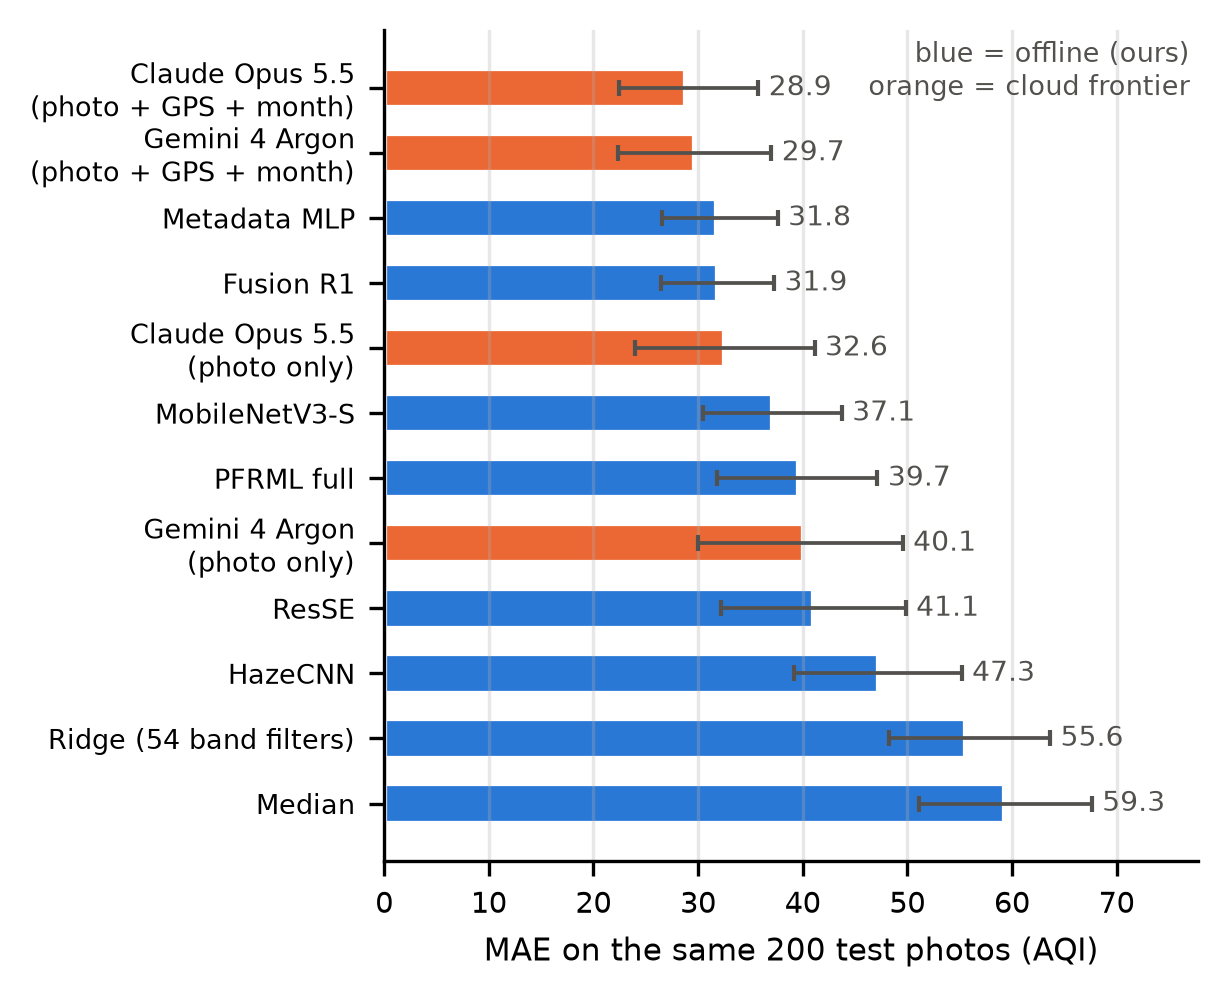
\includegraphics[width=\columnwidth]{figures/final_frontier_mae.png}
  \caption{MAE with 95\% station-bootstrap CIs on the same 200 test photos.
  Orange: frontier agents in the cloud; blue: our offline models.}
  \label{fig:frontiermae}
\end{figure}

\emph{First, given the same inputs, the frontier models are at least as
accurate as our best model.} With photo, GPS and month, Claude reaches an MAE of
28.9 and Gemini 29.7, against 31.9 for Fusion R1 on these photos. Neither
difference is significant ($-3.1$, CI [$-8.4$, 2.0], and $-2.2$, CI [$-7.9$,
3.3]), but both agents also have the highest rank correlation (0.86) and exact
category accuracy (55\% and 53\%) of all predictors. With the photo alone,
Claude (32.6) is level with Fusion R1 and better than our image-only
MobileNetV3-S (37.1), although that last difference narrowly misses
significance ($-4.5$, CI [$-11.2$, 0.8]). Gemini with the photo alone (40.1) is
significantly worse than Fusion R1.

\emph{Second, location helps the frontier models as much as it helps ours.}
Adding GPS and month lowers Claude's MAE by 3.7 (CI [0.3, 7.1]) and Gemini's by
10.3 (CI [6.3, 14.0]). Their written reasons show why. Even with the photo
alone, Claude often places the scene (``Japanese urban street, typically low
PM2.5''; ``a winter afternoon in southern Taiwan''; ``Looks like smog in a North
Indian city in winter''), so its photo-only answers already carry a location
prior read from architecture, signs and vegetation. With coordinates, both
agents recall local pollution climatology, for example ``near Anand Vihar in
East Delhi, where January PM2.5 is typically very high''. In other words, the
frontier models do what Fusion R1 does, combining a regional prior with haze
cues, but their prior comes from world knowledge instead of 8,176 training
photos. On the 39 unseen-region photos the frontier agents with metadata look
better still (30.5 and 33.3 against 39.7), but with so few photos the
intervals are very wide ($-9.3$, CI [$-30.7$, 6.4] for Claude) and we draw no
conclusion.

\emph{Third, they share a systematic bias.} All four frontier configurations
under-predict, by 15 to 33 AQI points on average, and they understate polluted
air more than our models do (Fig.~\ref{fig:frontierextra}a). Claude and Gemini
agree with each other more closely ($\rho=0.93$) than either agrees with the
truth (0.80 and 0.79), which suggests they apply the same visual heuristics.
Their self-reported confidence is informative, since photos answered with
higher confidence have lower errors, but Gemini reports systematically higher
confidence than Claude for similar errors (Fig.~\ref{fig:frontierextra}b).

\begin{figure*}[!t]
  \centering
  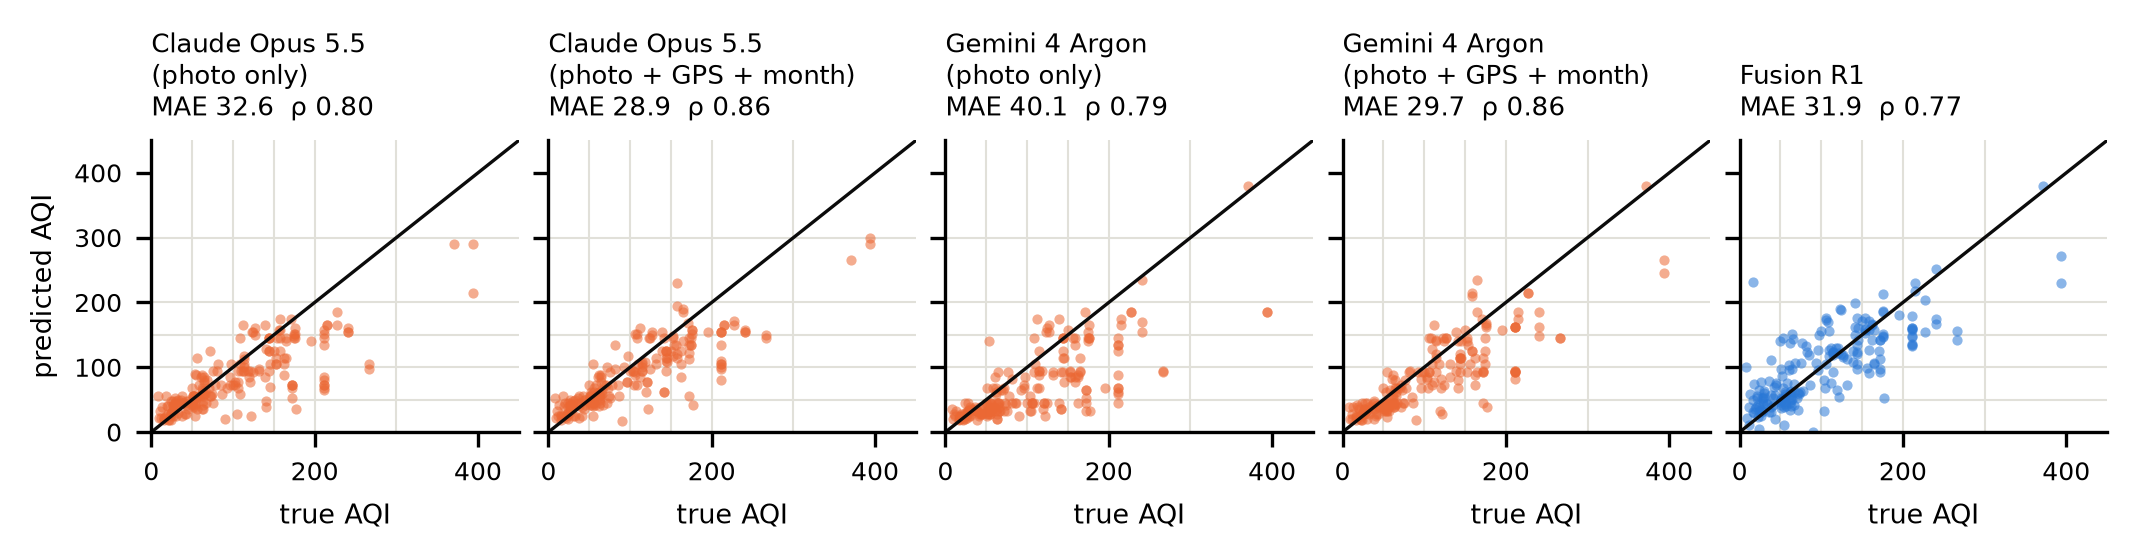
\includegraphics[width=\textwidth]{figures/final_frontier_scatter.png}
  \caption{Predicted versus true AQI on the 200 sample photos for the four
  frontier configurations and Fusion R1 ($\rho$: Spearman correlation).}
  \label{fig:frontierscatter}
\end{figure*}

\begin{figure*}[!t]
  \centering
  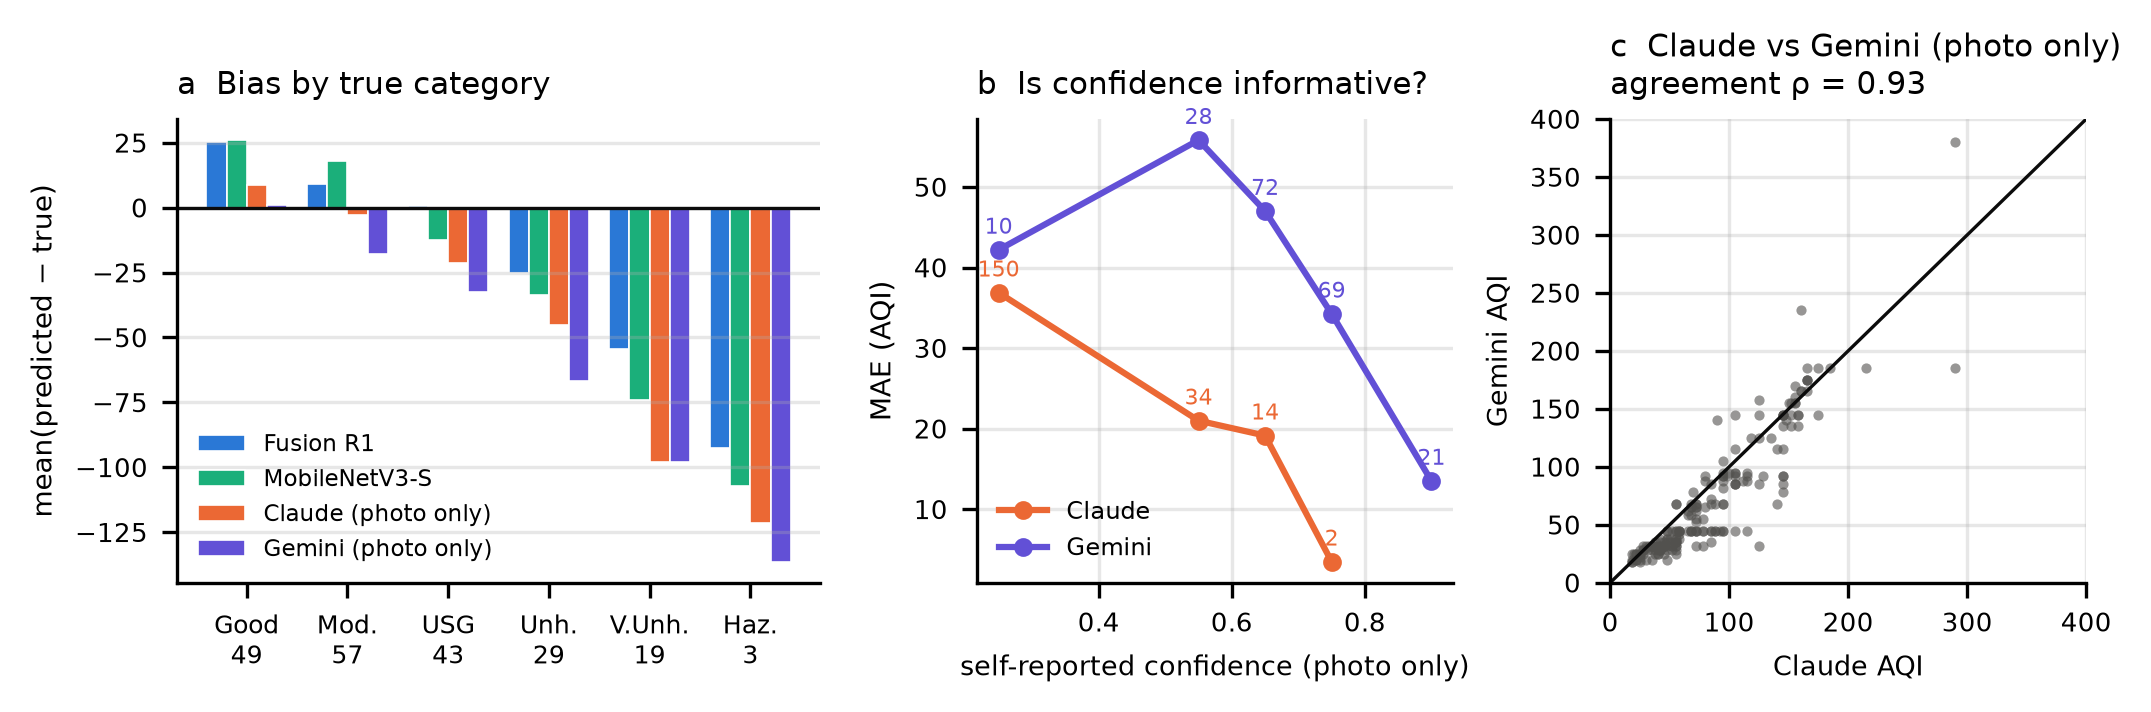
\includegraphics[width=\textwidth]{figures/final_frontier_extra.png}
  \caption{(a) Mean signed error by true category for our two best image
  models and the photo-only frontier agents (photo counts below the labels).
  (b) MAE against the agents' self-reported confidence (numbers: photos per
  bin). (c) The two agents agree with each other more than with the truth.}
  \label{fig:frontierextra}
\end{figure*}

\begin{figure*}[!t]
  \centering
  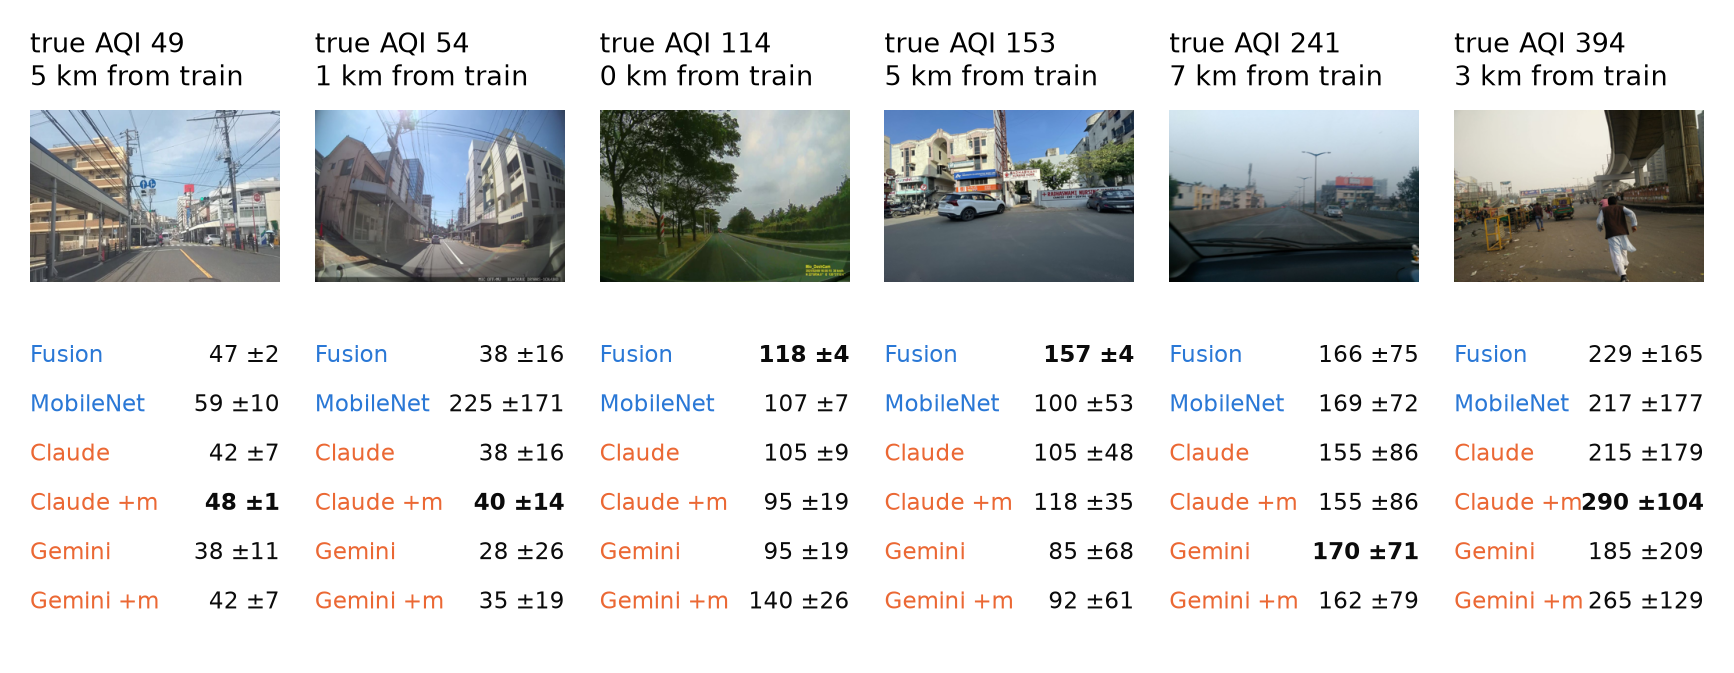
\includegraphics[width=\textwidth]{figures/final_frontier_samples.png}
  \caption{One sample photo per EPA category with the predictions of Fusion
  R1, MobileNetV3-S and the frontier agents (``+m'': with GPS and month).
  Absolute errors after $\pm$; bold marks the closest answer.}
  \label{fig:frontiersamples}
\end{figure*}

This accuracy comes at a cost. The median response time was 6.7\,s for Claude
and 16.2\,s for Gemini, and every query requires network connectivity,
transmits the user's image and location to a third party, and is billed per
request. Fusion R1 produces an estimate in 12\,ms on a single laptop CPU core.
Accuracy is therefore \emph{not} the argument for offline inference, since
frontier models already match our best model. The argument rests on privacy,
availability without connectivity, latency and cost, and
Section~\ref{sec:deploy} shows that our best model provides these on the
devices in common use.

\subsection{On-device footprint}
Table~\ref{tab:footprint} and Fig.~\ref{fig:footprint} report what each model
costs per photo, measured in notebook~5 on a single CPU core of an Apple M4 Pro
with PyTorch at batch size~1. Activation memory is the sum of all layer outputs
in one forward pass, an upper bound because a mobile runtime frees most of them
on the way.

\begin{table*}[!t]
  \centering
  \caption{On-device footprint per photo. FLOPs count a multiply-add as two
  operations. Latency: median of 100 runs, one CPU thread, batch size~1, Apple
  M4 Pro (a laptop core, faster than a phone core). Last column: change in full
  test-set MAE when the weights are stored in fp16 instead of fp32.}
  \label{tab:footprint}
  \setlength{\tabcolsep}{5pt}
  \begin{tabular}{lrccccccc}
    \toprule
    Model & Params & Input & GFLOPs & fp32 / fp16 / int8 (MB) & Activations (MB) & CPU latency (ms) & Test MAE & fp16 $\Delta$MAE \\
    \midrule
    Metadata MLP & 2,497 & 5 numbers & $<$0.001 & 0.01 / 0.005 / 0.002 & 0.001 & 0.01 & 36.8 & -- \\
    HazeCNN & 596,321 & 144$\times$192 & 1.87 & 2.28 / 1.14 / 0.57 & 20.6 & 9.4 & 51.4 & $-0.00$ \\
    ResSE & 1,192,865 & 144$\times$192 & 6.03 & 4.55 / 2.28 / 1.14 & 68.1 & 22.1 & 45.1 & $-0.11$ \\
    MobileNetV3-S & 1,518,881 & 224$\times$224 & 0.111 & 5.79 / 2.90 / 1.45 & 15.7 & 9.2 & 41.8 & $-0.01$ \\
    PFRML full & 2,107,331 & 224$\times$224 & 0.158 & 8.04 / 4.02 / 2.01 & 24.4 & 50.6 & 44.1 & $+0.04$ \\
    \textbf{Fusion R1} & 2,016,611 & 224$\times$224 + 5 & 0.158 & 7.69 / \textbf{3.85} / 1.92 & 24.4 & 11.5 & \textbf{35.6} & $+0.03$ \\
    \bottomrule
  \end{tabular}
\end{table*}

Three points matter for a phone. First, the parameter count is a poor guide
to cost. HazeCNN has the fewest weights of the image models, but it convolves at
full resolution and needs 17 times the FLOPs of MobileNetV3-S; ResSE needs 54
times. Second, Fusion R1 adds only 42\% FLOPs and about 2\,ms to MobileNetV3-S
for a 6-point gain in accuracy. PFRML has the same FLOPs as Fusion R1 but runs
four times slower, because its physics gate and attention pooling consist of
many small operations. Third, storing the weights in fp16 halves the download
to 3.85\,MB and changes the test MAE of every model by at most 0.11, so there is
no reason to ship fp32.

\begin{figure*}[!t]
  \centering
  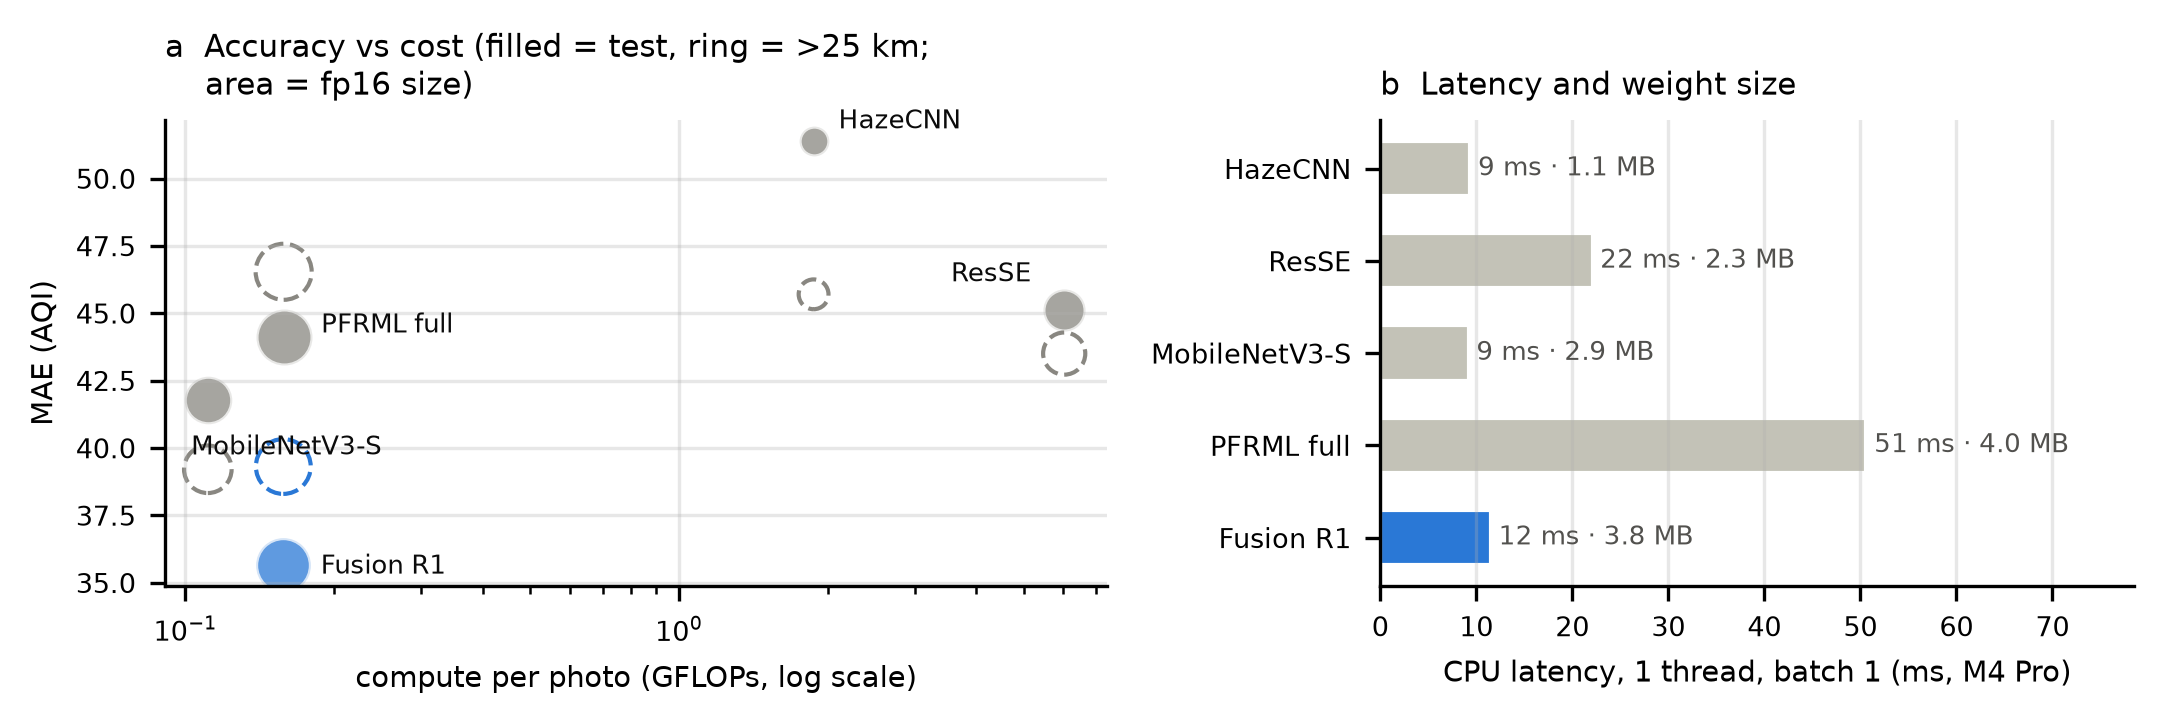
\includegraphics[width=\textwidth]{figures/final_footprint.png}
  \caption{(a) Test MAE (filled) and unseen-region MAE (dashed ring) against
  compute per photo; marker area is proportional to the fp16 weight size.
  (b) Single-thread CPU latency and fp16 size. Fusion R1 is the most accurate
  model and among the cheapest.}
  \label{fig:footprint}
\end{figure*}

\subsection{Where in the photo the models look}
To check that the networks use haze rather than incidental scene content, we
greyed out each cell of a $7\times7$ grid in 300 test photos and measured how
much the predicted AQI changed (Fig.~\ref{fig:occlusion}). Both Fusion R1 and
MobileNetV3-S draw about half of their sensitivity (49\% for Fusion R1) from
the three middle rows, where the horizon and distant buildings are, and the
least from the top row of open sky (9.5\%). That is what Eq.~\eqref{eq:scatter}
predicts: haze shows in how distant objects fade, not in the colour of the sky
alone. A grey sky by itself, as in the overcast photo of Fig.~\ref{fig:filters},
is weak evidence.

\begin{figure*}[!t]
  \centering
  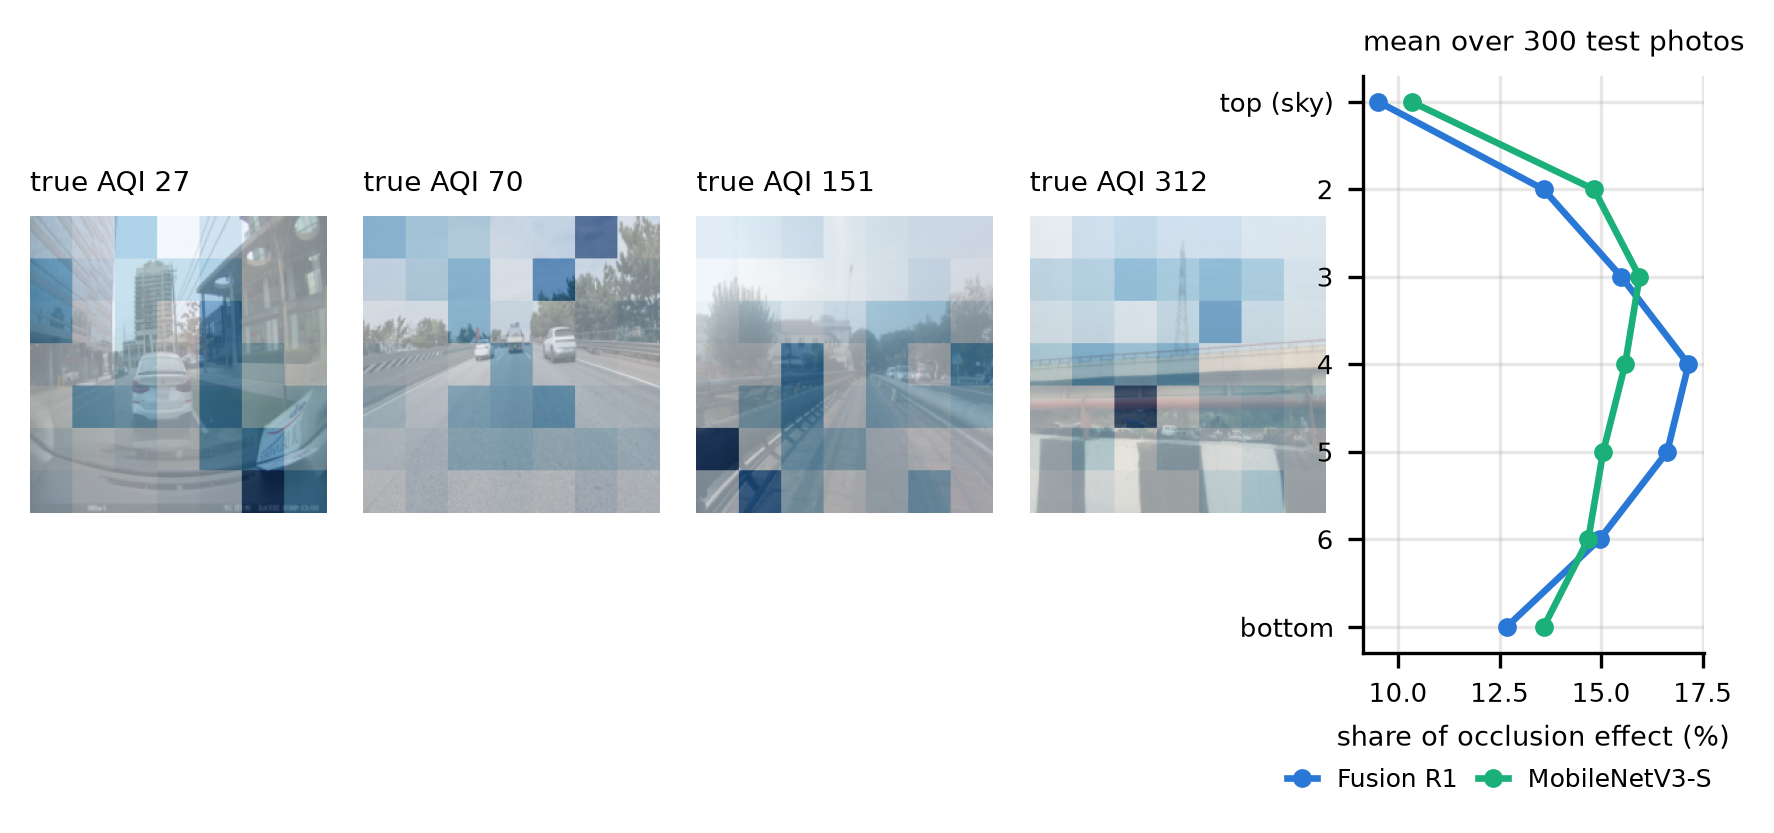
\includegraphics[width=\textwidth]{figures/final_occlusion.png}
  \caption{Occlusion sensitivity. Left: four test photos with Fusion R1's
  sensitivity map (darker blue = larger change in predicted AQI when that cell
  is hidden). Right: share of the total effect per image row, averaged over 300
  test photos.}
  \label{fig:occlusion}
\end{figure*}

% =====================================================================
\section{Which Model for 80\% of Users?}\label{sec:deploy}
% =====================================================================

Section~\ref{sec:mobile} set the target: a CPU-only octa-core phone with at
least 3\,GB of RAM and Android~11 or a recent iOS, which we estimate covers about
80\% of camera-phone users. Fig.~\ref{fig:devices} sets our models against it.

\begin{figure*}[!t]
  \centering
  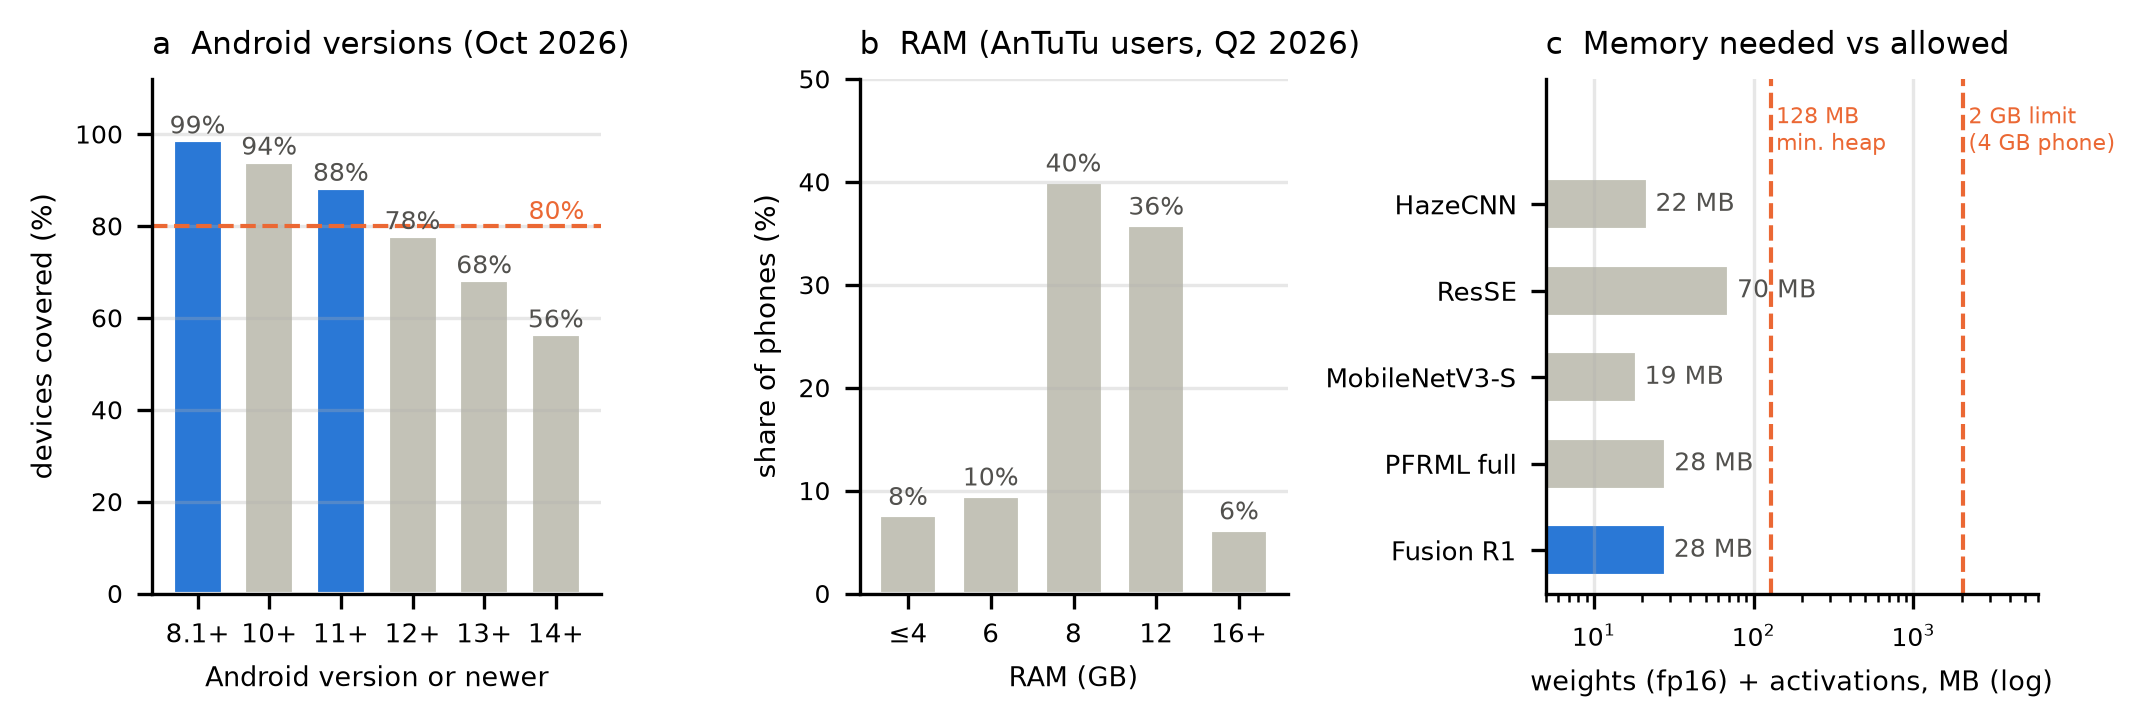
\includegraphics[width=\textwidth]{figures/final_devices.png}
  \caption{(a) Share of Google Play devices running each Android version or
  newer, October 2026 \cite{heise2026android}; LiteRT's CPU path runs on
  Android~8.1+. (b) RAM of phones tested with AnTuTu in Q2 2026
  \cite{antutu2026ram}, a sample biased towards new phones. (c) Memory each
  model needs (fp16 weights plus the activation upper bound) against the minimum
  app heap Android guarantees \cite{android16cdd} and the app limit on a 4\,GB
  phone \cite{android2026memorylimiter}.}
  \label{fig:devices}
\end{figure*}

\textbf{Memory.} Fusion R1 needs at most 28\,MB: 3.85\,MB of fp16 weights and an
upper bound of 24.4\,MB of activations. That is below even the 128\,MB minimum
Java heap Android guarantees every app, and about 1.4\% of the 2\,GB limit
Android~17 sets on a 4\,GB phone. Memory is therefore not a constraint for any
of our models, including the largest (ResSE, 70\,MB).

\textbf{Compute.} On low-end phones, compute speed rather than memory is the
binding constraint. MobileNetV3-Small
runs in 15.8\,ms on one big core of a 2016 Pixel~1 in fp32
\cite{howard2019mobilenetv3}. Fusion R1 needs 1.42 times its FLOPs, so on a
comparable core we expect a few tens of milliseconds; the Cortex-A73 to A76 big
cores of today's budget phones are roughly as fast as that 2016 core or faster. Even if a
low-end device were ten times slower than this estimate, the answer would
still arrive in well under a second. The from-scratch CNNs, by contrast, need
17--54 times the FLOPs of MobileNetV3-S, which by the same FLOP-proportional
reasoning means hundreds of milliseconds to nearly a second on such a core. These
are estimates; we did not measure on a phone.

\textbf{Software.} Fusion R1 uses only standard layer types (convolutions,
hard-swish, squeeze-and-excitation, layer normalisation, multi-head attention
and linear layers) that mobile runtimes such as LiteRT and Core ML provide,
although we have not converted it ourselves. LiteRT's CPU path runs on all
Android versions from 8.1, which cover 98.6\% of Google Play devices. No
accelerator is needed, so the model does not depend on an NPU, which LiteRT can
only use on Android~12 or newer with a 64-bit build and a supported chip
\cite{litert2026}.

\textbf{Recommendation.} We recommend deploying Fusion R1 as a 3.85\,MB fp16
file, converted to LiteRT on Android and Core ML on iOS. It fits the whole 80\% target
group with a wide margin and is the most accurate offline model. The app should
use the main head when the user allows location access, and fall back to the
built-in image-only head, at no extra cost, when location is denied. The
distance-aware switch of Section~\ref{sec:results} can be added by shipping
the coordinates of the 2,527 training stations (a few tens of kilobytes) and
computing the distance on the phone, once the 100~km boundary has been confirmed
on held-out data. Because of the regression to the middle, the app should show
the EPA category and its neighbour rather than a precise number, and state that
extreme smog and smoke episodes are underestimated. A frontier model could be
offered as an optional online second opinion, but only with the user's explicit
consent to upload the photo and location, since that gives up the privacy
the offline design is meant to protect.

% =====================================================================
\section{Discussion and Limitations}\label{sec:discussion}
% =====================================================================

\textbf{What the frontier comparison shows and does not show.} The comparison
uses 200 photos, one answer per photo and one version of each model, so a
single run of a different model version could move the numbers by a few points,
as the run-to-run variation of our own models showed. With 39 unseen-region
photos it cannot settle whether the frontier models generalise better than ours
far from training data. We cannot exclude that some PM25Vision photos, which
come from public sources, were part of the frontier models' training data,
although the labels are station readings that are not attached to the photos.
Giving the month instead of the date prevents looking up the exact reading, but
the models' knowledge of regional pollution is a legitimate prior, the same one
our metadata branch learns.

\textbf{Data limitations.} Each label is the reading of the nearest monitoring
station, which may be several kilometres away and may not match the photo's
exact hour, so part of every model's error is label noise. Three-quarters of the
test photos lie within 25~km of training photos, and Africa, Latin America and
Oceania together contribute only 8\% of the test set, so the regional estimates
there are uncertain. The test set has only 126 Hazardous photos and every model
underestimates them; this is the most important failure for a health
application.

\textbf{Camera domain.} PM25Vision contains dashcam and phone photos of many
kinds, which helps robustness, but we did not test on fresh photos from
current phones whose HDR and dehaze processing may differ. A field test in which
volunteers photograph the sky near reference monitors with several phone brands
is the natural next step.

\textbf{On-device validity.} All footprints were measured on a laptop CPU, and
phone latency was estimated from published figures and FLOP ratios. Converting
Fusion R1 to LiteRT and Core ML and timing it on a budget phone, for example
one with a Snapdragon~680 or Helio~G85, would replace the estimate with a
measurement.

\textbf{Responsible use.} A wrong ``Good'' during a smoke event could lead
someone to exercise outdoors. An app must therefore present the estimate as
indicative, report the category with its uncertainty, and point to official
readings when a network is available. Keeping inference on the phone also
means the user's location never leaves the device.

\textbf{Future work.} Beyond on-phone validation, three directions follow from
our results: learning the distance-aware switch on validation data;
distilling the frontier models' knowledge into the offline model by using their
photo + GPS + month answers as soft labels for unlabelled photos; and
tail-aware training (reweighting or quantile regression) to reduce the
underestimation of hazardous air.

% =====================================================================
\section{Conclusion}\label{sec:conclusion}
% =====================================================================

We asked whether a deep network small enough to run offline on an ordinary
phone can estimate air quality from a single street photo. On the global
PM25Vision benchmark, an image--metadata fusion network built on MobileNetV3-Small
provides a qualified affirmative answer. It reaches a test MAE of 35.6 AQI
points with 90\% of photos within one EPA category, keeps its accuracy in
regions without training stations where a location-only model collapses, and
is stable across training seeds (RQ1, RQ2). Handcrafted haze filters explain
little on their own; ImageNet pretraining and location metadata explain most of
the gain, and occlusion analysis shows that the networks read the fading of
distant objects rather than the colour of the sky.

Frontier models used zero-shot through their command-line agents are at least as
accurate when they receive the same inputs, and Claude matches our best model
from the photo alone, because both agents combine haze cues with world
knowledge about where and when the photo was taken (RQ3). The case for
offline inference is therefore not accuracy but privacy, availability without a
network, cost and latency. Fusion R1 delivers those with 2.0\,M parameters, a
3.85\,MB fp16 file, under 30\,MB of memory and an estimated few tens of
milliseconds per photo on a budget phone core, well within the hardware we
estimate 80\% of camera-phone users have (RQ4). The main open problem is the
systematic underestimation of hazardous air, which every model, offline or
frontier, shares.

\section*{Acknowledgment}
We thank the PM25Vision authors for releasing the dataset. Claude Code
(Anthropic) and the Antigravity CLI (Google) served as the command-line agents
in the experiment of Section~\ref{sec:frontier}.

\bibliographystyle{IEEEtran}
\bibliography{references}

\appendix

\subsection{Code and README}
All code is in the repository
\url{https://github.com/LitHaxor/acit-4620-projects} (branch \texttt{main}) and
in the code archive submitted with this report.

\textbf{Language and libraries.} Python~3.12 with PyTorch~2.14.1,
torchvision~0.29.1, scikit-learn~1.9.1, pandas~3.1.0, NumPy~2.5, Pillow~13.0,
Matplotlib~3.11 and JupyterLab~4.6 (exact versions in
\texttt{requirements.txt}). The frontier experiment additionally needs the
Claude Code CLI (2.1.330) and the Antigravity CLI (1.5.10), each logged in with
its own subscription.

\textbf{Platform.} All training and evaluation ran on an Apple M4 Pro laptop
(24\,GB unified memory) with the PyTorch \texttt{mps} backend; the code falls
back to CUDA or CPU automatically. Notebook~4 trains every model in about two
hours on this machine. Notebook~5 reuses notebook~4's checkpoints and runs in
about ten minutes, because the 800 frontier answers are stored in
\texttt{results/frontier/predictions.jsonl} and only missing answers are
requested again (the full frontier run took about 40 minutes).

\textbf{Setup.}
\begin{lstlisting}
python -m venv .venv && source .venv/bin/activate
pip install -r requirements.txt
python scripts/data/download_dataset.py   # PM25Vision -> datasets/
python -m pytest -q                        # unit tests
\end{lstlisting}

\textbf{Run order.}
\begin{lstlisting}
1.eda-image-datasets.ipynb       # audit, cleaning, EDA
2.feature-extraction.ipynb       # haze filters, band features, Ridge
3.example_train_test.ipynb       # HazeCNN / ResSE, grouped CV
4.models-eval-and-result.ipynb   # all models, test scores, seeds,
                                 # samples, verdict -> outputs/notebook4/
5.frontier-and-mobile-deployment.ipynb
                                 # Claude/Gemini CLI agents, Fusion heads,
                                 # occlusion, footprint, fp16, phone data,
                                 # every report figure -> results/, report/
cd report && tectonic final_report.tex
\end{lstlisting}

\textbf{Repository layout.}
\begin{lstlisting}
src/data/         cleaning, grouped splits, dataset, transforms
src/features/     18 haze statistics (PyTorch)
src/models/       baselines, MobileNetV3, DCM/Transformer,
                  PFRML prototypes, physics gate, fusion
train.py          cross-validation and training CLI
scripts/final_evaluation.py   one-shot test evaluation
scripts/experiments/          resumable CV queues
scripts/analysis/             reports, footprint, figures
configs/          YAML configs for every experiment
results/          tracked CSVs, curves, predictions,
                  frontier answers (results/frontier/),
                  footprint, phone-market facts
tests/            55 unit tests
\end{lstlisting}

\subsection{Frontier prompts}
Every call starts with the shared part, followed by one condition-specific
sentence and the shared suffix (\texttt{\{file\}}, \texttt{\{month\}},
\texttt{\{lat\}}, \texttt{\{lon\}} are filled in per photo):
\begin{lstlisting}
Open the image file {file} in the current directory and look at it. It is
a daytime street-level photo. Estimate the US EPA Air Quality Index (AQI)
computed from PM2.5 at the time and place it was taken (0-50 Good, 51-100
Moderate, 101-150 Unhealthy for Sensitive Groups, 151-200 Unhealthy,
201-300 Very Unhealthy, 301-500 Hazardous).
[photo only]  Judge only from what is visible: haze, visibility and
  contrast of distant objects, sky colour, light scattering.
[photo + GPS + month]  Context: the photo was taken in {month} at
  latitude {lat}, longitude {lon}. Combine the visible evidence with what
  you know about typical air quality at this place in this month.
Do not search the web and do not use any tool except opening the image.
Give a single best estimate (integer AQI), a confidence between 0 and 1,
and a reason of at most 25 words. Answer with the JSON object only.
\end{lstlisting}
Command lines (JSON schema omitted):
\begin{lstlisting}
claude -p "$PROMPT" --model claude-opus-5-5 --tools Read
  --allowedTools Read --strict-mcp-config --no-session-persistence
  --settings '{"disableAllHooks":true}' --output-format json
  --json-schema "$SCHEMA"
agy -p "$PROMPT" --model gemini-4-argon-medium --output-format json
  --json-schema "$SCHEMA" --print-timeout 170s
\end{lstlisting}

\subsection{Key code}
The differentiable haze-filter layer used by HazeCNN and ResSE
(notebook~3/4):
\begin{lstlisting}[language=Python]
class HazeFilters(nn.Module):
    # RGB (3 ch) -> RGB + 5 haze maps (8 ch)
    def forward(self, rgb):
        gray = rgb.mean(1, keepdim=True)
        hi = rgb.max(1, keepdim=True).values
        lo = rgb.min(1, keepdim=True).values
        dark = -F.max_pool2d(-lo, 7, 1, 3)
        sat = (hi - lo) / (hi + 1e-6)
        sx = torch.tensor([[-1.,0,1],[-2,0,2],[-1,0,1]],
                          device=rgb.device).view(1,1,3,3)
        edges = torch.sqrt(F.conv2d(gray, sx, padding=1)**2
                + F.conv2d(gray, sx.transpose(2,3), padding=1)**2)
        mu = F.avg_pool2d(gray, 7, 1, 3)
        con = (F.avg_pool2d(gray**2, 7, 1, 3) - mu**2).clamp(min=0).sqrt()
        return torch.cat([rgb, dark, sat, hi, edges, con], 1)
\end{lstlisting}
The Fusion R1 forward pass (\texttt{src/models/fusion.py}, simplified):
\begin{lstlisting}[language=Python]
feats = self.backbone(images)            # 4 MobileNetV3-S stages
fmap = self.head.neck(feats)             # DCM: [B, 224, 14, 14]
chi, _ = self.head.transformer(fmap)     # [B, 224]
m = self.metadata_mlp.forward_features(meta)  # [B, 32]
reg = self.head.reg_head(chi, extra_feat=m)   # AQI / 100
aux = self.aux_reg_head(chi)                  # image-only head
\end{lstlisting}

\end{document}
